% Tento soubor nahraďte vlastním souborem s obsahem práce.
%=========================================================================
% Autoři: Michal Bidlo, Bohuslav Křena, Jaroslav Dytrych, Petr Veigend a Adam Herout 2019

% Pro kompilaci po částech (viz projekt.tex), nutno odkomentovat a upravit
%\documentclass[../projekt.tex]{subfiles}
%\begin{document}

\chapter{Úvod}
V současnosti vývoj webových aplikací výrazně pokročil. Moderní webové stránky a aplikace kladou stále náročnější požadavky nejen na technologickou a funkční stránku, ale~také~na~vizuální prezentaci. Vzhledem k rostoucí složitosti realizace rozsáhlých projektů vznikají řešení, jejichž cílem je zrychlit vývoj a usnadnit práci vývojářů.

Pro tyto účely byla vytvořena platforma Oidis\footnote{https://docs.oidis.io/}, která zahrnuje několik součástí poskytujících kompletní prostředí pro vývoj webových aplikací. Oidis nabízí vývojářům sadu nástrojů pro automatizaci, testování a správu DevOps\footnote{DevOps je přístup ke koordinaci vývoje a provozu softwaru, který zrychluje a zjednodušuje dodávání aplikací díky automatizaci a průběžné spolupráci.} projektů. Součástí platformy jsou také~základní šablony a komponenty, které pokrývají běžně požadovanou funkcionalitu ve~většině současných webových aplikací a další rozšiřující možnosti.

Přestože platforma poskytuje pevný základ, na němž může být webová aplikace vystavěna, současné projekty kladou vysoké nároky také na grafickou stránku výsledného řešení. Proto je vhodné využít grafické editory, které výrazně zjednodušují a urychlují návrh frontendu (z anglického \textit{frontend}, v kontextu této práce část webové aplikace, se kterou uživatel přímo interaguje -- tedy vizuální rozhraní). Tyto editory nabízejí vizuální prostředí, v němž~lze skládat komponenty, nastavovat jejich vlastnosti, okamžitě sledovat výsledek a~exportovat generovaný kód, aniž by bylo nutné jej psát ručně. Tento přístup urychluje implementaci a zároveň umožňuje zapojit do návrhu uživatelského rozhraní i programátory, jejichž primární specializací není vývoj frontendu.

Cílem této diplomové práce je ve spolupráci se společností Oidis Solutions\footnote{https://www.oidis.org} vytvořit grafický editor, který umožní návrh uživatelského rozhraní webových aplikací s využitím knihovny Bootstrap\footnote{https://getbootstrap.com}. Navrhované řešení má nahradit stávající nástroj Bootstrap Studio\footnote{https://bootstrapstudio.io}, který je v současnosti využíván při vývoji projektů na platformě Oidis. Přestože tento nástroj dokáže urychlit implementaci uživatelského rozhraní, vykazuje řadu nedostatků, které snižují efektivitu práce vývojářů. Z tohoto důvodu vznikl požadavek na vytvoření vlastního řešení, které bude plně kompatibilní s platformou Oidis a zároveň bude lépe odpovídat konkrétním potřebám jejích uživatelů.

Práce je strukturována tak, aby postupně představila teoretický základ, navazující analýzu, návrh řešení a jeho následnou realizaci a ověření. Kapitola \ref{Teorie} popisuje možné architektury webových aplikací, shrnuje principy návrhu uživatelských rozhraní, přístup \textit{low-code} vývoje a přehled nástrojů pro tvorbu webových rozhraní, včetně řešení využívaného platformou Oidis. Kapitola \ref{Oidis} popisuje platformu Oidis, její účel a architekturu, a zároveň představuje přístupy k vývoji multiplatformních aplikací. Na tuto část navazuje kapitola \ref{Editory}, v~níž~je analyzován současný stav a formulovány požadavky na nový grafický editor, který by dokázal nahradit stávající řešení a lépe odpovídal specifickým potřebám platformy. Návrhové aspekty aplikace jsou řešeny v kapitole \ref{Navrh}, kde je popsán uživatelský workflow, struktura editoru a způsob jeho technického propojení s platformou Oidis. Implementační část práce je obsažena v kapitole \ref{Implementace}, která popisuje použitá technická řešení a postup vývoje. Závěrečná kapitola \ref{Testovani} se věnuje testování výsledné aplikace a ověření funkčnosti klíčových částí editoru.


\chapter{Moderní webové aplikace, jejich architektura a přístupy k návrhu uživatelského rozhraní}
\label{Teorie}
Moderní web již nepředstavuje pouze soubor statických webových stránek, ale je tvořen především webovými aplikacemi, které poskytují interaktivní služby koncovým uživatelům. Webová aplikace je chápána jako klient–server aplikace, která využívá webový prohlížeč jako~klientský program a komunikuje se serverovou částí prostřednictvím internetové nebo~intranetové sítě~\cite{WebApps}. Na rozdíl od klasického webu založeného na statickém obsahu, webová aplikace prezentuje dynamicky přizpůsobený obsah na základě požadovaných parametrů, sledování chování uživatelů a bezpečnostních požadavků.

Současné webové aplikace se stávají komplexními systémy, které podporují podnikové procesy, integrují se s externími systémy a musí být schopny rychle reagovat na změny v~konkurenčním prostředí~\cite{Shirani2004}. Tyto aplikace proto musí být přístupné z různých zařízení, adaptivní a responzivní, zahrnovat podporu přirozených vstupů (dotyk, hlas, GPS, senzory), integraci sociálních sítí, možnost škálování v cloudu, odolnost proti výpadkům, snadnou údržbu a vysokou spolehlivost~\cite{Ciliberti2013}. Webové aplikace nejsou pouze prostředkem pro prezentaci informací, ale poskytují interaktivní funkce a dosahují stejné úrovně složitosti jako tradiční desktopové programy.


\section{Architektura webových aplikací}
\label{Architektury}
Posun od statických dokumentů k interaktivním aplikacím zásadně změnil způsob návrhu i vývoje webových řešení. Webové aplikace dnes zpracovávají uživatelské vstupy v reálném čase, pracují s databázemi, autentizací a autorizací uživatelů a často integrují další externí služby a systémy. Výsledkem je výrazný nárůst funkční i architektonické složitosti, který~klade nové požadavky na jejich návrh, strukturu a udržovatelnost~\cite{WebApps}.

V této sekci je uveden přehled architektur frontendové části webových aplikací. Jsou zde popsány monolitická architektura~\ref{Monoliticka}, komponentní architektura~\ref{Komponentni} a microfrontendová (z anglického \textit{microfrontend}) architektura~\ref{MikroFrontendy}. Rozdíly mezi jednotlivými architekturami určují strukturu projektu a přístup k vývoji, čímž přímo ovlivňují i způsoby, jakými je navrhováno uživatelské rozhraní. Projekt Oidis Studio, vytvořený v rámci této diplomové práce, je vyvíjen na Oidis Frameworku a jeho účelem je podpora vývoje dalších aplikací na tomto frameworku (z anglického framework). Volba přístupů k návrhu uživatelského rozhraní proto přímo vychází z architektury Oidis Frameworku~\ref{Oidis}, na kterém je projekt postaven. Přístupy k návrhu UI jsou podrobně popsány v sekci~\ref{UiPristupy} a aktuální přístup a~nástroje, použité při vývoji projektů na frameworku Oidis, v sekci~\ref{AktualniNastroje}.

\subsection{Monolitická architektura}
\label{Monoliticka}
Monolitická architektura představuje řešení, v~němž je celá aplikace vyvíjena jako jediná rozsáhlá kódová báze sdílená mezi všemi vývojáři. Aplikace je typicky strukturována do~tří
vrstev -- prezentační, obchodní a~perzistenční. Veškerá funkcionalita se~nasazuje jako jeden nedělitelný celek, takže přidání nové funkce nebo oprava chyby vyžaduje opětovné sestavení celé aplikace včetně všech jejích služeb. Monolitické nasazení zároveň představuje jediný bod selhání -- pokud aplikace spadne, přestanou být dostupné všechny její služby najednou~\cite{Monolith}.

Monolitické frontendy vznikají z~jedné kódové báze, na~které
smysluplně pracuje jen~jeden tým -- jakmile do~téže kódové báze
přispívá týmů více, začnou si vzájemně překážet. Ve~větších organizacích bývá odpovědnost za~aplikaci navíc rozdělena
podle technologií mezi~více týmů -- jeden tým spravuje frontend,
další tým či týmy backend (z~anglického \textit{backend}). Vývoj funkce procházející oběma vrstvami proto vyžaduje koordinaci napříč týmy, například změnu sdíleného rozhraní si týmy musí nejprve dohodnout, naplánovat do~svých sprintů a~funkce je dokončená až ve~chvíli, kdy svou část odevzdá poslední z~nich. Komunikační režie přitom roste s~velikostí
zapojených týmů a~stává se brzdou vývoje~\cite{MicrofrontensGeers}.

Navzdory uvedeným omezením nabízejí monolitické frontendy také řadu
výhod, díky kterým byly velmi rozšířené. V~malém týmu odpovědném
za~celý projekt si každý vývojář udržuje přehled o~celé funkcionalitě, nové funkce vznikají rychle a~diskuze nad nimi probíhají neformálně a~přímo, bez nutnosti svolávat formální schůzky a~sestavovat detailní specifikaci. Monolitická aplikace navíc vyžaduje pouze jeden aplikační server, jeden buildovací proces a~jedinou CI/CD pipeline pro celý projekt, takže technická režie i~nasazení jsou jednodušší tím, že aplikace se sestaví a~zveřejní jako jeden celek~\cite{MicrofrontensGeers}.

\subsection{Komponentní architektura}
\label{Komponentni}
Komponentově orientovaná architektura představuje v současnosti jeden z nejrozšířenějších přístupů k organizaci moderních webových aplikací na straně uživatelského rozhraní. Základní myšlenkou tohoto přístupu je považovat komponenty za elementární stavební jednotky aplikace. Tento princip je využíván v populárních frontendových frameworkech, jako~jsou React\footnote{https://react.dev}, Vue\footnote{https://vuejs.org} nebo Angular\footnote{https://angular.dev}, a lze jej považovat za standard při vývoji rozsáhlých a dynamických webových systémů~\cite{ComponentArch}.

Popis komponentní architektury představený v této sekci vychází z~\cite{ComponentArch}, podle něhož je komponenta chápána jako samostatně zapouzdřený funkční modul uživatelského rozhraní, který disponuje vlastní strukturou, definicí stylu, aplikační logikou a řízením vlastního stavu. Díky těmto vlastnostem je komponenta opakovaně použitelná, nezávislá na konkrétním kontextu aplikace a může být flexibilně kombinována s ostatními komponentami podle~aktuálních požadavků systému.

Komponentová architektura rozděluje webovou aplikaci na množství provázaných funkčních celků. Jednotlivé komponenty spolu komunikují prostřednictvím jasně definovaných rozhraní a přenosem dat, čímž se minimalizuje logická závislost mezi moduly. Tento přístup eliminuje problémy typické pro tradiční návrh založený na stránkách, jako je duplicitní kód, obtížná údržba nebo omezená možnost rozšiřování aplikace. Výsledkem je lepší udržovatelnost, škálovatelnost a dlouhodobá stabilita systému.

Komponentová architektura představuje z pohledu vývoje vysoce strukturovaný, modulární a volně provázaný vývojový model, který výrazně zjednodušuje návrh i implementaci rozsáhlých webových aplikací. Důležitou součástí tohoto modelu je podpora lokálního vykreslování a postupného načítání obsahu -- aplikace nemusí být vykreslována jako celek, ale pouze v částech potřebných v daném okamžiku. Díky mechanismům líného načítání přispívá to ke snížení paměťových nároků, zlepšení odezvy aplikace a zvýšení uživatelského komfortu, zejména 
u rozsáhlých systémů~\cite{ComponentArch}.

V praxi je komponentová architektura často podporována souborem doplňkových technologií a návrhových principů. Mezi nejvýznamnější patří využití virtuálního DOM pro~optimalizaci vykreslovacího procesu, jednosměrný tok dat pro zachování konzistence změn stavu nebo mechanismy kompozice aplikace, které umožňují izolaci funkcionalit a opětovné použití kódu. Načítání komponent na vyžádání prostřednictvím konfigurovatelných cest dále přispívá ke snížení počáteční zátěže aplikace~\cite{ComponentArch}.

Pro systematický návrh a organizaci komponent se v praxi využívá princip atomického designu, který hierarchicky organizuje komponenty podle jejich složitosti a funkční úrovně: atomy představují základní HTML prvky, molekuly jsou skupiny atomů tvořící jednoduchou funkční jednotku, organismy tvoří komplexní sekce rozhraní, šablony definují rozložení stránky a stránky představují konkrétní instance šablon s reálným obsahem. Dalším běžně~uplatňovaným vzorem je oddělení prezentačních a kontejnerových komponent, kdy prezentační komponenty zodpovídají výhradně za vizuální zobrazení a kontejnerové komponenty zajišťují přístup k datům a aplikační logice. S tím úzce souvisí princip jediné odpovědnosti, podle něhož by každá 
komponenta měla mít jeden jasně vymezený účel, což~zvyšuje čitelnost 
a znovupoužitelnost kódu~\cite{ComponentDriven}. 

Komponentově orientovaný přístup zvyšuje udržovatelnost aplikace, protože izolované části uživatelského rozhraní snižují riziko nechtěných vedlejších efektů a usnadňují dlouhodobý rozvoj i úpravy systému. Také přináší lepší testovatelnost, jelikož jednotlivé komponenty lze testovat samostatně, což podporuje systematické testování a omezuje vznik regresních chyb. Oproti monolitnímu přístupu umožňuje efektivnější opětovné využití kódu. Modularita komponent výrazně zlepšuje spolupráci mezi týmy, protože umožňuje paralelní vývoj a nezávislou práci na různých částech uživatelského rozhraní a usnadňuje průběžnou integraci a nasazení změn~\cite{ComponentDriven}. 

Celkově komponentově orientovanou architekturu je možné považovat za klíčový přístup pro~návrh moderních webových aplikací, který nejen zlepšuje řízení vývoje a údržbu systému, ale zároveň efektivně podporuje výkon a kvalitu uživatelského rozhraní v komplexních a dynamických prostředích.

\subsection{Architektura microfrontendů}
\label{MikroFrontendy}
Microfrontendy představují architektonický styl, ve kterém je komplexní frontendová aplikace systematicky složena z více menších, autonomních frontendových aplikací~\cite{MicroFrontends}. Každý microfrontend může být vyvíjen, testován a nasazován nezávisle různými vývojovými týmy. Tento přístup rozšiřuje principy mikroslužbové architektury (z anglického \textit{microservices}, architektonický styl, v němž je aplikace rozdělena do sady malých, nezávisle nasaditelných služeb) do oblasti frontendu a vytváří distribuovaný systém uživatelských rozhraní. Ekosystém microfrontendů se obvykle skládá z několika klíčových komponent, které spolupracují mezi sebou~\cite{MicroFrontends}:

\begin{itemize}
    \item \textbf{Kontejnerová aplikace} funguje jako hostitelské prostředí, které spravuje a integruje více microfrontendů. Typicky zajišťuje směrování, autentizaci a sdílené služby.
    \item \textbf{Microfrontendové aplikace} fungují jako samostatné prvky implementující konkrétní obchodní funkcionalitu, přičemž jejich složitost se může výrazně lišit.
    \item \textbf{Integrační vrstva} poskytuje komunikační mechanismy a sdílené služby mezi jednotlivými microfrontendy. Tyto vrstvy často implementují architekturu řízenou událostmi, která v aktivních podnikových prostředích zpracovává velké objemy zpráv mezi~komponentami.
    \item \textbf{Směrovací systémy} řídí navigaci v aplikaci a určují, který microfrontend má obsluhovat konkrétní aplikační cesty. Pokročilé implementace směrování podporují strategie líného načítání a přednačítání, které predikují navigační chování uživatelů a~tím~podstatně snižují vnímané doby načítání.
\end{itemize}

 Architektura microfrontendů podle~\cite{MicrofrontensGeers} vychází
z~principu nezávislého nasazování, kdy~je každý microfrontend vyvíjen,
testován a~nasazován samostatně, bez nutnosti konzultace s~ostatními
týmy. Technologická nezávislost umožňuje týmům volit nástroje
a~technologie nejvhodnější pro jejich konkrétní oblast -- jednotlivé
týmy nesdílejí knihovny ani frameworky a~mají plnou kontrolu nad
vlastním technologickým zásobníkem. To~usnadňuje postupné zavádění
a~ověřování nových technologií v~izolované části aplikace bez nutnosti
vytvářet rozsáhlý migrační plán pro~celý systém. Jednotlivé microfrontendy lze následně integrovat do~výsledné aplikace
různými způsoby: serverovou kompozicí, klientskou kompozicí (s~využitím
iframe nebo webových komponent) či kombinací obou přístupů.

\section{Přístupy k návrhu UI pro webové aplikace}
\label{UiPristupy}

Návrh uživatelského rozhraní webových aplikací představuje samostatnou a odborně náročnou činnost, která by neměla být redukována pouze na implementační fázi vývoje. Řada nedostatků v kvalitě uživatelského rozhraní vzniká v důsledku neformálního a nekoordinovaného postupu návrhu. Pokud návrh UI vzniká během implementace, bez jasně definovaných kroků a bez srozumitelného předání návrhu vývojářům, často dochází k rozdílům mezi~zamýšleným návrhem a výslednou podobou rozhraní~\cite{Design}.

Z tohoto důvodu by měl být návrh uživatelského rozhraní vytvořen jako samostatný výstup designéra ještě před samotnou implementací aplikace. Tento návrh slouží nejen~jako~vizuální představa výsledného rozhraní, ale také jako komunikační prostředek mezi designéry, vývojáři a dalšími účastníky projektu. Jasně formulovaný návrh umožňuje sjednotit představu o chování aplikace, její struktuře a způsobu interakce s uživatelem~\cite{Design}.

Proces návrhu UI je obvykle rozdělen do několika etap, které umožňují postupné zpřesňování návrhu. V počátečních fázích se návrh zaměřuje na celkovou koncepci rozhraní, mentální model uživatele a základní strukturu navigace. Následují fáze, ve kterých je návrh rozpracován do konkrétních obrazovek, jejich vzájemných vazeb a detailního uspořádání prvků. Tento postup umožňuje nejprve řešit koncepční otázky a teprve poté přistupovat k~detailům, čímž se snižuje riziko zásadních změn v pozdějších fázích vývoje~\cite{Design}.

Kvalitní návrh UI by měl existovat nezávisle na konkrétní formě jeho technické realizace~\cite{Design}. V praxi návrh uživatelského rozhraní obvykle začíná ve specializovaných grafických nástrojích, jako jsou Figma\footnote{https://www.figma.com/}, Sketch\footnote{https://www.sketch.com/} nebo Adobe XD\footnote{https://www.adobe.com/}, které umožňují rychle sestavit vizuální návrhy a ladit jejich chování pomocí prototypů. Tyto nástroje nejsou přímo propojeny s implementací a nepracují s reálnými komponentami -- designéři v nich pracují výhradně s vizuálními prvky a své návrhy následně předávají vývojářům k implementaci.

Způsob, jakým je návrh UI následně realizován, se může lišit v závislosti na použitých nástrojích a vývojových přístupech. Návrh může být implementován ručním psaním kódu značkovacího jazyka a skriptů, vývojáři mohou využívat předpřipravené komponenty a šablony. Návrh může sloužit jako podklad pro nástroje, které automaticky generují uživatelské rozhraní (takový přístup je popsán v sekci~\ref{Autogenerate}), nebo může být přímo vytvářen a upravován pomocí vizuálních editorů.

\subsection{Manuální programování uživatelského rozhraní}
Ruční programování uživatelského rozhraní webových aplikací je tradiční přístup, při němž je výsledné rozhraní implementováno přímo pomocí standardních webových technologií, jako jsou HTML, CSS a JavaScript. Tento způsob vývoje předpokládá, že vývojář překládá návrh UI (např. z prototypu nebo designu vytvořeného v grafickém nástroji) do zdrojového kódu, přičemž má plnou kontrolu nad strukturou, stylem i chováním jednotlivých prvků uživatelského rozhraní.

V rámci tohoto způsobu vývoje je dnes běžné využívat komponentní přístup, kdy jsou jednotlivé prvky UI rozděleny do znovupoužitelných stavebních bloků. Tento způsob umožňuje efektivnější správu složitějších rozhraní, podporuje konzistenci designu a zkracuje dobu vývoje při úpravách a rozšiřování aplikace~\cite{ComponentArch}.

Dále vývojáři často využívají frameworky a knihovny, které jim poskytují předpřipravené komponenty a funkce, a tím urychlují implementaci běžných prvků UI. Na rozdíl od~knihoven, které vývojáři integrují dle potřeby a mají plnou kontrolu nad architekturou aplikace, frameworky obvykle předdefinují strukturu projektu a vyžadují dodržování určitých pravidel a vzorců, což může vést k vyšší komplexnosti, ale zároveň usnadňuje organizaci rozsáhlejších aplikací~\cite{ManualImplementation}. Mezi nejčastěji používané frameworky patří například React, Angular, Vue. Dále se využívají frontendové knihovny poskytující sadu hotových komponent, jako Bootstrap nebo Material UI\footnote{https://mui.com/material-ui/}, které usnadňují tvorbu responzivních a konzistentních rozhraní.

\subsection{Koncept low-code}
\label{LowCode}
Koncept low-code představuje způsob tvorby softwaru, který minimalizuje potřebu ručního programování a využívá vizuální rozhraní, automatickou generaci kódu a modelově řízený přístup. Vývoj aplikací probíhá prostřednictvím grafických nástrojů, kde jsou komponenty skládány pomocí techniky \textit{drag-and-drop} (přesun prvků po obrazovce pomocí myši), a výsledná implementace je automaticky generována z vytvořených modelů. Tento přístup umožňuje zapojení uživatelů bez hlubších znalostí programování, kteří se však orientují v~dané doméně a dokážou vytvářet či upravovat aplikace. Platformy low-code tak přispívají ke zrychlení vývoje, zefektivnění spolupráce mezi programátory a doménovými specialisty a k řešení nedostatku kvalifikovaných vývojářů. Typické rysy tohoto přístupu zahrnují vizuální návrh, agilní iterativní vývoj, podporu integrace s datovými a službovými vrstvami a nasazení v prostředí cloudu~\cite{LowCodeKirikova}.

Podle~\cite{LowCodePlatforms} \textit{low-code development} označuje způsob vývoje softwaru, který se opírá o vizuální modelování, konfiguraci a předdefinované komponenty spíše než o klasické psaní kódu. Podstatou přístupu low-code je využití vizuální reprezentace aplikace, datových struktur a~vazeb mezi nimi, kterou systém následně převádí do odpovídajícího programového kódu. 

Po analýze zdrojů~\cite{LowCodeKirikova,LowCodePlatforms} lze identifikovat několik hlavních výhod přístupu low-code. Tento přístup především výrazně zrychluje vývoj, protože umožňuje sestavovat a nasazovat aplikace podstatně rychleji než při tradičním ručním programování. Zároveň podporuje zapojení neprogramátorů do procesu tvorby aplikací, čímž se snižuje závislost na vysoce kvalifikovaných vývojářích. Další významnou výhodou je snížení nákladů na vývoj, jelikož~není nutné ručně psát rozsáhlé množství zdrojového kódu. Platformy využívající přístup low-code rovněž podporují agilní způsob vývoje díky možnosti rychlých úprav, iterací a prototypování. Současně podporují integraci s dalšími systémy a datovými zdroji a obvykle obsahují nástroje pro připojení k \textit{API} (Application Programming Interface\footnote{https://www.ibm.com/think/topics/api}), databázím a externím službám.

Přístup low-code má však také řadu nevýhod~\cite{LowCodeKirikova,LowCodePlatforms}:

\begin{itemize}
    \item{\textbf{Omezená rozšiřitelnost a flexibilita.} Možnosti uživatele jsou často vymezeny množinou předdefinovaných komponent a uzavřenou architekturou, která neumožňuje snadné doplňování vlastních funkcí. Rozšíření funkcionality nebo provádění změn mimo rámec platformy je v proprietárních systémech často obtížné nebo zcela nemožné.}
    \item{\textbf{Závislost na konkrétním dodavateli.} Aplikace vyvinuté na jedné low-code platformě bývají obtížně přenositelné na jinou kvůli proprietárnímu formátu kódu a uzavřenému datovému modelu.}
    \item{\textbf{Obtížná integrace složitější logiky.} Low-code nástroje jsou efektivní pro běžné scénáře, avšak pokročilé nebo netypické logické procesy často přesahují jejich vizuální schopnosti. Implementace složitější obchodní logiky či nestandardních datových toků obvykle vyžaduje ruční programování mimo vizuální rozhraní.}
    \item{\textbf{Nedostatečná podpora testování a verzování.} Mnoho low-code platforem neposkytuje dostatečné možnosti pro automatizované testování, kontinuální integraci ani~verzovací systémy.}
    \item{\textbf{Bezpečnostní a provozní rizika.} Vzhledem k tomu, že většina low-code platforem funguje v cloudovém prostředí, mohou vznikat problémy týkající se bezpečnosti, ochrany dat a správy přístupových práv, jelikož zpracování probíhá v externí infrastruktuře, kterou organizace nemá plně pod kontrolou.}
\end{itemize}

\subsection{Automatické generování kódu z návrhu UI}
\label{Autogenerate}
Přestože na trhu existuje řada nástrojů, které podporují návrh a vývoj uživatelských rozhraní odděleně, většina z nich neposkytuje mechanismy pro přímý převod nebo plynulý přechod práce designérů k vývojářům. V posledních letech se objevila řada nástrojů zaměřených na převod návrhových artefaktů do kódu, jejichž hlavním cílem je minimalizovat rozdíl mezi návrhem a frontendovým vývojem a rovnou umožnit export HTML a CSS kódu. Vývojáři však uvádějí, že navzdory této možnosti bývá generovaný kód kvůli své~kvalitě jen~zřídka používán přímo~\cite{GeneratedDesign}.

Nástroje pro převod návrhu do kódu lze rozdělit do tří skupin: zásuvné moduly pro~nástroje tvorby návrhu UI, jako jsou Sketch nebo Figma, nástroje pro převod návrhového souboru do kódu a nástroje pro převod obrazů do kódu. Zásuvné moduly rozšiřují funkcionalitu nástrojů Sketch nebo Figma a převádějí konkrétní součásti návrhu, například komponenty nebo stránky, do kódu v cílovém programovacím jazyce. Druhou skupinu tvoří nástroje, které přijímají jako vstup přímo návrhový soubor odpovídajícího nástroje a převádějí jej do kódu. Poslední skupinu představují nástroje, které převádějí snímky obrazovky ve formátu JPEG do HTML a SCSS kódu, často založeného na knihovně Bootstrap~\cite{GeneratedDesign}.

Za účelem řešení problému převodu návrhů uživatelského rozhraní do programového kódu bylo navrženo několik přístupů založených na odlišných technikách. Tyto přístupy se~liší zejména způsobem, jakým analyzují vstupní návrh a jak generují výsledný kód.

Jednou ze skupin jsou heuristicky založené techniky, jejichž cílem je dekompozice a interpretace vstupních dat. Tyto přístupy kombinují metody, jako je optické rozpoznávání znaků (OCR), počítačové vidění a heuristické postupy, za účelem identifikace jednotlivých prvků uživatelského rozhraní. OCR je využíváno především pro detekci textových elementů, zatímco techniky počítačového vidění slouží k identifikaci vizuálních charakteristik, jako jsou hrany, rohy a základní tvary. Na základě těchto informací je následně vytvářena struktura komponent, která slouží jako podklad pro generování kódu. Nevýhodou tohoto přístupu může být nižší kvalita výsledného kódu a jeho omezená čitelnost a upravitelnost~\cite{GeneratedDesign}.

Další skupinu tvoří \textit{end-to-end} techniky, které se snaží pokrýt celý proces převodu návrhu do kódu jedním modelem bez explicitního rozdělení na dílčí kroky. Tyto přístupy typicky kombinují konvoluční neuronové sítě (CNN) a rekurentní neuronové sítě (RNN). CNN zajišťuje extrakci příznaků ze vstupního obrazu a převod návrhu do vnitřní reprezentace, zatímco RNN modeluje sekvenční strukturu odpovídající výslednému kódu. End-to-end přístupy umožňují generovat kód přímo ze vstupního návrhu, avšak jejich omezením je vysoká náročnost na trénovací data a obtížná generalizace na nové, dosud neviděné návrhy~\cite{GeneratedDesign}.

Samostatnou skupinu představují techniky založené na detekci objektů, které využívají algoritmy pro rozpoznávání jednotlivých komponent v návrhu. Tyto metody identifikují prvky uživatelského rozhraní na základě extrakce příznaků a učících algoritmů a následně je organizují podle jejich vzájemných prostorových vztahů. Výsledkem je hierarchická struktura rozhraní, která slouží jako základ pro generování kódu cílové platformy~\cite{GeneratedDesign}.

Jiný přístup k návrhu uživatelského rozhraní je založen na automatické generaci frontendového kódu s využitím principů responzivního webového designu. Na příkladu nástroje popsaného v~\cite{MobileFirst} je představen odlišný způsob automatizace realizace návrhu UI. Nástroj umožňuje vytvořit vizuální návrh uživatelského rozhraní nejprve pro platformu telefonu a následně automaticky generuje vizuální návrhy pro další platformy spolu s odpovídajícím kódem. Tento postup vychází ze zásady \textit{mobile-first}, kdy je návrh optimalizován pro~nejmenší zařízení, protože rozšiřování obsahu pro větší obrazovky je jednodušší než~jeho dodatečné omezování.

Automatická generace kódu je založena na souboru principů responzivního webového designu, které pokrývají návrh navigace, rozložení, obrázků, formulářů a textu. Dodržování těchto principů je klíčové pro zachování správného chování rozhraní napříč různými velikostmi obrazovek a pro udržení použitelnosti aplikace~\cite{MobileFirst}.

Hodnocení popsaného nástroje v~\cite{MobileFirst} potvrdilo, že uživatelská rozhraní vytvořená pomocí tohoto nástroje dodržují principy responzivního designu a zachovávají použitelnost na~všech podporovaných zařízeních. Autoři zároveň uvádějí, že nástroj představuje počáteční řešení, které je možné dále rozšiřovat o pokročilejší možnosti stylování, práci s typografií, barvami, rozestupy a předdefinovanými šablonami.

\section{Aktuální nástroj využitý platformou Oidis a dostupné alternativy}
\label{AktualniNastroje}
Sekce~\ref{UiPristupy} představila přístupy, které lze aplikovat při převodu návrhu aplikace vytvořeného designérem do výsledného kódu. Byl představen manuální přístup, automatické generování kódu založené na rozpoznávání znaků a prvků uživatelského rozhraní nebo~pomocí neuronových sítí, a také low-code přístup. V případě automatického generování kódu nebo~použití platforem low-code se jedná o pokročilejší techniky, které mohou výrazně urychlit vývoj aplikací. Automatické generování kódu přímo z návrhového designu, jak bylo uvedeno v~sekci~\ref{Autogenerate}, však často vede k nižší kvalitě výsledného kódu a k omezené čitelnosti a upravitelnosti. To nemusí představovat zásadní problém u jednoduchých aplikací, které~se~dále neupravují, avšak u dlouhodobě udržovatelných aplikací s měnícími se požadavky během vývoje jde o významné omezení. Z tohoto pohledu low-code platformy lépe odpovídají potřebám takto vyvíjených aplikací. Pro dosažení optimálních výsledků je však nutné správně vymezit části systému, ve kterých je vhodné tento přístup uplatnit.

Většina současných low-code platforem podle~\cite{LowCodePlatforms} je navržena jako komplexní prostředí, které umožňuje tvorbu, správu a provoz celé aplikace prostřednictvím grafického rozhraní. Tyto systémy obvykle zahrnují moduly pro návrh uživatelského rozhraní, definici logiky, práci s daty, integraci externích služeb i samotné nasazení aplikace. Takové platformy tedy~poskytují vývojářům možnost řídit celý životní cyklus aplikace od návrhu po údržbu, bez nutnosti využívat tradiční programovací nástroje.

Platforma Oidis již v současné době poskytuje komplexní prostředí určené pro správu, údržbu a DevOps automatizaci projektů. Nabízí vývojářům širokou sadu nástrojů pro testování, správu verzí, nasazování aplikací a řízení životního cyklu softwaru. Je tedy primárně zaměřena na provozní a infrastrukturní část vývoje, ale nenabízí nástroje určené pro rychlou realizaci návrhu frontendové části aplikací.

Proto je vhodné aplikovat low-code přístup pouze na konkrétní část vývojového procesu, a to na vývoj frontendu. Oblast návrhu UI je pro využití low-code principů mimořádně vhodná -- práce s technologiemi HTML, CSS a JavaScript je vysoce strukturovaná a~umožňuje snadné převádění návrhů do vizuálního prostředí, které může automaticky generovat odpovídající kód. Vizuální návrhové prostředí tak uživateli umožní intuitivní tvorbu komponent a rozhraní s možností jejich následného exportu jako plnohodnotného kódu kompatibilního s projekty v rámci platformy Oidis.

Pro zvýšení efektivity práce a zajištění systematického přístupu k vývoji 
uživatelského rozhraní je při vývoji aplikací na platformě Oidis využívána 
knihovna Bootstrap, která poskytuje předdefinované komponenty a styly. Pro vizuální návrh komponent s využitím této knihovny platforma v současnosti 
používá grafický editor, jehož funkcionalita však není pro~potřeby platformy Oidis plně dostačující. Tato sekce se proto zaměřuje na dostupné grafické editory, které umožňují low-code přístup v kontextu návrhu webových aplikací s~podporou knihovny Bootstrap. Představena je aplikace Bootstrap Studio, která je v současnosti využívána platformou Oidis, spolu s několika dostupnými alternativami.

\subsection{Bootstrap Studio}
\label{BootstrapStudio}
Bootstrap Studio\footnote{https://bootstrapstudio.io/} je desktopová aplikace, která funguje plně offline a je distribuována formou jednorázové licence. Hlavním cílem je vizuální návrh pomocí předpřipravených HTML komponent nebo komponent knihovny Bootstrap s generováním HTML obsahujícího Bootstrap třídy nebo vestavěné CSS styly. Aplikace podporuje Bootstrap ve verzích 4 a 5.

Podle oficiální dokumentace~\cite{BootstrapStudioDocs} je aplikace postavena na principu vizuálních uprav. Návrhy stránek se vytvářejí přetahováním předpřipravených HTML tagu nebo Bootstrap komponent z katalogu dostupných elementu pomoci techniky drag-and-drop. Následně aplikace dovoluje upravit styly vytvořených elementů. Bootstrap Studio generuje čistý kód v~jazycích HTML, CSS a JS, který je optimalizovaný a podporovaný ve všech webových prohlížečích. 

Dokumenty vytvořené v Bootstrap Studio se nazývají \textit{Designy}. Každý takový dokument lze uložit jako soubor s příponou \texttt{.bsdesign}, který obsahuje veškerý obsah projektu, včetně~kódu, obrázků a fontů. Obsah vytvořeného návrhu je možné exportovat jako složku obsahující běžné soubory HTML, CSS, JS a obrázky~\cite{BootstrapStudioDocs}. Exportovaný kód je navržen tak, aby byl čitelný, dobře formátovaný a umožňoval další ruční úpravy. Aplikace umožňuje import existujících HTML/CSS/JS souborů, které následně převádí do vnitřního formátu. Aplikace nabízí \textit{live preview}, poskytuje možnost publikace designu na hosting a nabízí nástroje pro úpravu HTML, CSS, SASS a JS přímo uvnitř prostředí aplikace. 

Přesto jsou generované výstupy i vnitřní reprezentace projektu stále více orientovány na~tvorbu statických stránek navržených jako celek, bez přímé podpory pro propojení s~aplikační logikou nebo backendovými službami. Editor sice umožňuje importovat nebo ručně upravovat kód, ale veškerá komplexnější funkcionalita, která přesahuje rámec samotných vizuálních prvků, musí být doplněna mimo prostředí editoru.

Tento přístup komplikuje práci zejména u projektů založených na komponentovém přístupu (viz. sekci~\ref{Komponentni}), což je případ platformy Oidis, kde je aplikace tvořena menšími opakovaně použitelnými bloky namísto celé stránky. Omezením je také interní formát, v~němž~jsou návrhy ukládány -- ten znesnadňuje následné úpravy existujících komponent i~udržení shody mezi návrhovou verzí a skutečnou implementací. Navíc chybí podpora pro~systematickou identifikaci grafických prvků a nástroje, které by automatizovaly propojení mezi návrhem a logikou aplikace, což nutí vývojáře opakovaně provádět některé kroky ručně.

\subsection{Pinegrow}

Pinegrow\footnote{https://pinegrow.com} funguje primárně jako desktopová aplikace, ale nabízí i online režim pro práci s projekty. Na rozdíl od 
Bootstrap Studia nepracuje s interním formátem -- projekty jsou uloženy jako běžné HTML a CSS soubory, které lze otevírat a upravovat v libovolném externím editoru. Pinegrow tyto soubory aktivně sleduje a změny provedené v externím editoru automaticky detekuje a promítá do vizuálního návrhu~\cite{PinegrowDocs}. Díky tomu lze Pinegrow používat souběžně s jiným kódovým editorem, přičemž oba nástroje zůstávají synchronizované. Aplikace nabízí vizuální tvorbu stránek pomocí přetahování komponent, ovládání parametrů jednotlivých komponent 
a zároveň podporuje přímé úpravy HTML a CSS kódu. Aplikace má plnou 
podporu knihovny Bootstrap~\cite{PinegrowDocs}.

Export probíhá přímým uložením projektu jako složky se standardními soubory HTML a CSS, ke kterým může být doplněna aplikační logika. Tento přístup je vhodný zejména pro projekty, u nichž je celý frontend navrhován jako sada stránek a kde není vyžadována hlubší integrace s aplikačním frameworkem.

Přestože Pinegrow nabízí oproti Bootstrap Studiu výhodu v podobě práce se standardními soubory a podpory externího editoru, jeho přístup k návrhu zůstává orientován na~tvorbu celých stránek. V kontextu platformy Oidis, kde jsou aplikace tvořeny množinou menších opakovaně použitelných komponent s vazbou na framework, Pinegrow nepřináší oproti Bootstrap Studiu zásadní výhodu.

Celkově je Pinegrow silný nástroj pro vizuální návrh a rychlé prototypování malých až~středně velkých projektů, který poskytuje flexibilitu při práci s HTML/CSS a Bootstrap komponentami. Jeho přístup je však omezený pro scénáře 
vyžadující komponentový přístup nebo propojení s logikou aplikace. Podle informací uvedených v dokumentaci~\cite{PinegrowDocs} je tento~nástroj prezentován jako jednoduchý a produktivní způsob návrhu statických webových stránek.

\subsection{LayoutIt}

LayoutIt\footnote{https://layoutit.com} je primárně webová aplikace pro návrh základních struktur stránek s využitím knihovny Bootstrap. Uživatelé mohou komponenty přetahovat na plátno a vizuálně skládat jejich rozvržení, přičemž generovaný HTML kód lze stáhnout a následně využít v jiných projektech.

Aplikace je vhodná pro rychlé prototypování a návrh vizuální struktury stránek, ale~nenabízí pokročilé možnosti úprav jednotlivých komponent uvnitř editoru. Přímá editace kódu je omezena a neexistuje možnost importovat existující HTML soubory či projekty pro~jejich následnou vizuální úpravu. Pro účely platformy Oidis je LayoutIt nevhodný. Absence importu existujících souborů a omezené možnosti úprav komponent vylučují jeho použití v komponentovém přístupu, kde je nezbytná opakovaná vizuální editace a synchronizace s~kódem projektu.

\section{Shrnutí}
Moderní web je dnes tvořen především webovými aplikacemi, které na rozdíl od statických webových stránek prezentují dynamicky generovaný obsah a kladou důraz na interakci s~uživateli. Rostoucí složitost webových aplikací vedla k postupnému přechodu od jednoduchých monolitických architektur, popsaných v sekci~\ref{Monoliticka}, k pokročilejším architektonickým přístupům, které jsou běžně využívány také u desktopových aplikací.

Při návrhu uživatelského rozhraní webové aplikace je před samotnou implementací obvykle designérem vytvořen návrhový prototyp, který je následně převáděn vývojáři do programového kódu. Pro realizaci komplexních řešení jsou využívány frontendové frameworky a knihovny předpřipravených komponent, které usnadňují vývoj a zároveň definují architekturu i výslednou strukturu aplikace. V sekci~\ref{LowCode} je představen alternativní přístup low-code. Přestože jsou platformy založené na tomto principu primárně zaměřeny na vývoj celé aplikace prostřednictvím grafických nástrojů, je možné využít jejich dílčí části orientované na návrh frontendové části aplikace pomocí vizuálních editorů. Použití těchto nástrojů umožňuje zachovat tradiční přístup k vývoji webové aplikace s plnou kontrolou nad aplikační logikou a současně usnadnit převod návrhu uživatelského rozhraní do výsledného kódu.

Z tohoto důvodu je při vývoji webových aplikací na platformě Oidis v současnosti využíván nástroj Bootstrap Studio, který propojuje vizuální modelování s automatickým generováním kódu. Při jeho používání se ukázalo, že dokáže výrazně zkrátit dobu potřebnou k~realizaci návrhu i k následným úpravám komponent při změnách jejich designu. Z analýzy trhu grafických editorů podporujících knihovnu Bootstrap, představených v sekci~\ref{AktualniNastroje}, Bootstrap Studio nejlépe odpovídá architektuře a způsobu použití frameworku Oidis. Ostatní dostupná řešení se buď snaží pokrýt příliš široké spektrum technologií bez hlubší specializace na Bootstrap, jsou primárně zaměřena na tvorbu statických webových stránek, nebo~podporují pouze počáteční návrh uživatelského rozhraní s omezenými možnostmi další editace a aplikace změn mimo vlastní prostředí.

Přestože Bootstrap Studio nabízí široké možnosti a je přímo zaměřeno na práci s knihovnou Bootstrap, je navrženo pro kompletní vývoj uživatelského rozhraní výhradně ve~svém vlastním prostředí (viz~\ref{BootstrapStudio}). Z tohoto důvodu vznikl požadavek na vytvoření nového editoru, který zachová hlavní výhody Bootstrap Studia, avšak bude lépe odpovídat specifickým potřebám platformy Oidis.

\chapter{Platforma Oidis} 
\label{Oidis}
Webové aplikace dnes dosahují srovnatelné úrovně složitosti jako tradiční desktopové programy. To platí zejména při řešení specifických úloh v dané doméně, při práci s komplexní aplikační logikou, při přístupu k různým periferiím a při integraci s externími systémy. Jak~bylo uvedeno v sekci~\ref{UiPristupy}, komplexnější aplikace nejsou obvykle vyvíjeny od nuly, ale~jsou stavěny s využitím knihoven a frameworků, které urychlují jejich tvorbu a umožňují systematický přístup k vývoji. Frameworky definují architekturu aplikace, kterou je nutné dodržovat, i způsob, jakým má být aplikace navržena a implementována.

Podobně jako low-code platformy popsané v sekci~\ref{LowCode}, které řídí celý proces vývoje aplikace prostřednictvím grafických nástrojů, existují také platformy využívající tradičnější přístup k vývoji webových aplikací. Jednou z těchto platforem je platforma Oidis.

V této práci je termín \textit{platforma Oidis} používán jako označení souhrnu všech nástrojů, které tato platforma zahrnuje. Její hlavní součástí je Oidis Framework, chápaný v kontextu této práce jako softwarový balík obsahující zdrojový kód, knihovny a nástroje určené pro~vývoj multiplatformních aplikací, který je podrobně popsán v sekci~\ref{OidisFramework}. Platforma dále zahrnuje sadu nástrojů zajišťujících plnou automatizaci procesů sestavení a nasazení aplikací (\textit{CI/CD, DevOps}). Součástí platformy jsou rovněž nástroje pro monitoring koncových aplikací, podporu komunikace se zákazníky, správu procesních a pracovních postupů, řízení projektů a další nástroje podporující efektivní správu vývoje softwaru.

Platforma Oidis vznikla jako soubor nástrojů s cílem urychlit vývoj koncových aplikací a~snížit náklady na jejich vývoj i provoz. Jejím hlavním záměrem je tvorba multiplatformních aplikací (podrobněji popsáno v sekci~\ref{Multiplatformni}). Základní charakteristikou těchto aplikací je jednotné uživatelské prostředí a konzistentní funkčnost bez ohledu na používané zařízení či~operační systém. Vzhled aplikace se může lišit pouze v závislosti na velikosti displeje nebo~rozměrech aplikačního okna.

Ukázkou takových řešení vytvořených na platformě Oidis jsou například:
\begin{itemize}
\item Konfigurační a diagnostické aplikace pro mikropočítače.
\item Nástroje pro kalibraci kamerových čoček.
\item Frontend pro generování modelů typu \textit{Speech-to-Text} a \textit{Speech-to-Intent}.
\item Aplikace pro konfiguraci parametrů řízení motorů.
\item Drag-and-drop IDE pro generování OpenVX kódu.
\item Nástroje pro odbavování zásilek v logistice.
\item Systém pro tisk a zpracování čárových kódů.
\item Vzdálená komunikace a správa IoT zařízení.
\item Systém chytré domácnosti včetně podpory HW.
\item Aplikace pro podporu autistických dětí.
\item Rozšíření CRM systémů o agendu splátkových kalendářů.
\item Podnikové systémy pro elektronické zpracování poptávek ve stavebnictví.
\item Aplikace pro evidenci docházky.
\end{itemize}

Tento výčet ukazuje, že moderní webové aplikace se stávají komplexními nástroji určenými k řešení specifických a často technicky náročných problémů. To klade vysoké nároky nejen na technologické možnosti používaných frameworků, ale také na samotný proces návrhu a vývoje těchto aplikací. Představené aplikace jsou ve většině případů realizovány jako~webové aplikace běžící primárně v internetovém prohlížeči a využívající externí nástroje, služby nebo výpočetní skripty. Zároveň jsou některé z nich vyvíjeny pro více platforem nebo mají možnost rychlé adaptace na další platformy podle aktuálních potřeb. Z~tohoto důvodu je v následující sekci~\ref{Multiplatformni} vhodné popsat možné přístupy k vývoji multiplatformních aplikací.

\section{Přístupy k multiplatformnímu vývoji}
\label{Multiplatformni}
Z pohledu obchodních požadavků je multiplatformní vývoj klíčovou vlastností moderních aplikací. Umožňuje prosadit aplikaci mezi širší skupinu uživatelů a zajistit její využití na~různých zařízeních, což je v mnoha případech velmi žádoucí. Publikace~\cite{CrossPlatformSurvey, Taxonomy} prezentují multiplatformní vývoj především z pohledu mobilních zařízení. Podle~\cite{CrossPlatformSurvey} je většina aplikací v mobilních obchodech vyvíjena pomocí přístupu označovaného jako \textit{nativní}. Tento vývojový přístup využívá programovací jazyky, nástroje a vývojová prostředí specificky určená pro daný operační systém. Například vývoj nativních aplikací pro platformu iOS vyžaduje znalost vývojového prostředí Xcode\footnote{https://developer.apple.com/xcode/} a programovacích jazyků Swift\footnote{https://www.swift.org} nebo Objective-C\footnote{https://developer.apple.com/documentation/objectivec}, zatímco aplikace pro Android vyžadují znalost Android Studia\footnote{https://developer.android.com/studio} a jazyků Java či Kotlin\footnote{https://kotlinlang.org}. V~důsledku toho nelze aplikace vyvinuté pro Android nasadit ani spustit na zařízení s iOS a~naopak. Každá nová podporovaná platforma proto vyžaduje vývoj aplikace od nuly. Vývoj pro různé platformy vyžaduje znalost všech příslušných technologií, a každá nová funkce nebo oprava chyb musí být implementována zvlášť pro každou platformu.

Alternativou k tomuto přístupu jsou řešení, která umožňují uspokojit stejné obchodní potřeby napříč více platformami. Cílem je minimalizovat náklady na vývoj a údržbu sjednocením technologií, vývojových cyklů a samotných aplikací. Ačkoliv motivace k přijetí multiplatformního přístupu mohou být různé, rozpočet, čas a dostupné znalosti jsou v literatuře~\cite{CrossPlatformSurvey} uváděny jako nejčastější důvody, proč preferovat multiplatformní vývoj před~tradičním nativním vývojem.

Nezávisle na tom, zda se jedná o mobilní zařízení, či jiné platformy, hlavní myšlenka multiplatformních aplikací zůstává stejná: vyvinout aplikaci jednou a umožnit její spuštění kdekoli~\cite{CrossPlatform}. Podle~\cite{CrossPlatformSurvey} je konečným cílem vývoje mobilních aplikací napříč platformami dosáhnout výkonu srovnatelného s nativními aplikacemi a zajistit jejich běh na co největším počtu platforem.

Různé publikace odlišně klasifikují přístupy k multiplatformnímu vývoji. Například~\cite{CrossPlatform} uvádí následující kategorie: kompilovaný, interpretovaný, komponentní, webový, pomocí virtuálních strojů, za běhu (\textit{runtime}), modelově řízený, low-code, cloudový a kombinovaný. Podle~\cite{CrossPlatformSurvey} lze přístupy rozdělit na hybridní, interpretované, křížově kompilované, modelově řízené a progresivní webové aplikace (\textit{PWA}). Další členění~\cite{Taxonomy} rozlišuje pět základních kategorií multiplatformního vývoje: webový, hybridní, interpretovaný, křížově kompilovaný a~modelově řízený přístup. V dalších sekcích uvádím nativní, webový a hybridní přístup. Některá z výše uvedených členění tyto základní kategorie rozšiřují, případně podle různých publikací spadají do odlišných kategorií.

\subsection{Nativní aplikace}
Nativní aplikace jsou vyvíjeny přímo pro konkrétní operační systém a využívají jeho vlastní API a knihovny. Tento přístup poskytuje vysoký výkon, spolehlivou integraci se systémem a plný přístup ke všem periferiím, včetně specializovaných funkcí, které nejsou dostupné v~jiných typech řešení~\cite{CrossPlatformSurvey}.

Hlavním problémem nativního přístupu je nízká přenositelnost. Pokud má být aplikace dostupná na více platformách, je nutné ji vyvíjet a udržovat v několika samostatných verzích. V praxi to znamená vznik více implementací téže funkcionality, které je nutné průběžně synchronizovat. Z tohoto důvodu je nativní přístup vhodný především tam, kde je kladen důraz na maximální výkon nebo kde aplikace využívá systémové funkce, které jiné přístupy nedokážou zajistit.

Příkladem takového řešení je Telegram\footnote{https://telegram.org}, 
který disponuje samostatnými nativními implementacemi pro každou podporovanou platformu -- desktopová aplikace je napsána v~C++, klient pro Android v jazyce Java a aplikace pro iOS a macOS v jazyce Swift. Důvodem jsou rozdíly v platformových API pro zvuk a video hovory, hardwarově akcelerované kryptografické operace specifické pro každý operační systém a odlišné mechanismy 
integrace s~nativními notifikačními systémy. Tyto systémové prvky fungují na každé platformě odlišně a~nelze je spolehlivě zastřešit jedinou sdílenou vrstvou bez ztráty výkonu nebo funkcionality.

\subsection{Webové aplikace}
\label{Pwa_sec}
Webové aplikace lze nahlížet z různých perspektiv. Jedním pohledem je jejich chápání jako~rozšíření klasických webových stránek, druhým pak přístup k nim jako k multiplatformním aplikacím, které využívají technologie typické pro webový vývoj, a jejichž běh i~zobrazení zajišťuje webový prohlížeč.

Podle~\cite{Taxonomy} jsou webové aplikace vyvíjeny pomocí webových technologií, jako jsou HTML, JavaScript a CSS. Nevyžadují instalaci, neboť jsou přístupné prostřednictvím URL adresy zadané ve webovém prohlížeči. Mezi jejich hlavní výhody patří relativně snadný vývoj díky použití standardizovaných webových technologií. Veškeré zpracování aplikační logiky obvykle probíhá na serveru a do koncového zařízení je přenášeno pouze uživatelské rozhraní určené k vykreslení. Údržba aplikace je zjednodušena tím, že aktualizace aplikace i dat jsou prováděny centrálně na serveru. Aplikace může být vyvinuta jednou a následně provozována na různých platformách prostřednictvím webových prohlížečů.

Na druhou stranu, webové aplikace nejsou standardně distribuovány prostřednictvím aplikačních obchodů a jejich používání je podmíněno aktivním připojením k internetu. Další nevýhodou je omezený přístup k softwarovým a hardwarovým funkcím zařízení, jako~jsou například kamera nebo GPS senzory. Tato omezení však nevyplývají z technických nedostatků webových technologií, ale ze záměrně uplatňovaných bezpečnostních pravidel webových prohlížečů. Právě tato omezení mohou komplikovat provoz náročnějších systémů, které~pak musí využívat doplňkové mechanismy nebo nástroje obcházející omezení prohlížeče. Dalším problémem webových aplikací je rozdílné chování v jednotlivých webových prohlížečích, což nutí vývojáře věnovat značné úsilí testování a odstraňování těchto rozdílů.

Z pohledu webových aplikací jako multiplatformního přístupu publikace~\cite{CrossPlatform} popisuje tento směr jako vývoj mobilních aplikací pomocí webových technologií s využitím specifického HTML prohlížeče pro každou platformu. Důsledkem tohoto přístupu je, že výsledné aplikace jsou zpravidla méně efektivní než nativní aplikace a zároveň nemají shodný vzhled a chování odpovídající nativnímu uživatelskému rozhraní dané platformy.

Publikace~\cite{Taxonomy} nahlíží na tento přístup v kontextu multiplatformního vývoje, zejména se~zaměřením na mobilní aplikace, jako na vývoj aplikací založených na webových technologiích, které jsou rozšířeny o mechanismy umožňující přístup k funkcím zařízení, jako jsou kamera nebo senzory. Toho je dosaženo pomocí obalových vrstev nad nativními API. Autoři uvádějí především platformu PhoneGap (dnes známou jako Apache Cordova\footnote{https://cordova.apache.org}), která~umožňuje načítat webové aplikace do nativních aplikací a zpřístupňovat jim vybrané hardwarové a softwarové funkce zařízení. Dále jsou zmiňována webová běhová prostředí určená pro~vývoj webových aplikací napříč mobilními platformami, která lze chápat také jako lehké mobilní webové prohlížeče nebo mobilní desktopová prostředí. Tyto přístupy však již svými vlastnostmi více odpovídají kategorii hybridních aplikací než čistě webovým aplikacím.

Další kategorií, kterou autoři uvádějí v rámci webového přístupu~\cite{Taxonomy}, jsou progresivní webové aplikace (\textit{Progressive Web Apps, PWA}). Na úrovni konceptů podle~\cite{Pwa} jsou PWA postaveny na souboru deseti základních principů. \textit{Progresivnost} vychází z principu postupného zlepšování, kdy aplikace nabízí základní funkcionalitu i na méně výkonných zařízeních nebo~v~prohlížečích bez plné podpory moderních technologií, zatímco na výkonnějších platformách poskytuje rozšířené funkce. \textit{Responzivní design} zajišťuje optimální zobrazení obsahu na různých typech zařízení a velikostech obrazovek. \textit{Možnost instalace aplikace přímo z prohlížeče}, bez nutnosti využití tradičních aplikačních obchodů, přibližuje webové aplikace tradičním nativním řešením. PWA jsou dále navrženy tak, aby \textit{fungovaly i bez připojení k~internetu}, a to díky ukládání dat a prostředků do mezipaměti a využití technologie \textit{Service Workers}.

Progresivní aplikace může působit téměř nerozeznatelně od nativní aplikace díky \textit{vzhledu a chování} podobnému nativním řešením. \textit{Zajištění aktuálnosti obsahu} je dosaženo kombinací offline režimu a synchronizace dat na pozadí, což umožňuje poskytovat uživateli jak~dostupnost bez připojení, tak i čerstvá data po opětovném připojení. \textit{Bezpečnost} je zajištěna povinným využitím protokolu HTTPS. Progresivní webové aplikace jsou rovněž snadno \textit{dohledatelné vyhledávači}, neboť jsou založeny na běžných webových stránkách s rozšířenou funkcionalitou. Umožňují také opětovné zapojení uživatele pomocí \textit{push notifikací}, podobně jako u nativních aplikací. Posledním principem je možnost \textit{snadného sdílení obsahu} prostřednictvím URL adres, přičemž některé platformy umožňují, aby se instalovaná PWA automaticky otevřela při návštěvě odpovídajícího odkazu.

Z technologického hlediska jsou podle~\cite{Pwa, Pwa_webdev} klíčovým prvkem progresivních aplikací jsou Service Workers. Jedná se o programy v jazyce JavaScript, které běží na pozadí odděleně od hlavního rozhraní aplikace a nemají přímý přístup k objektovému modelu dokumentu (DOM). Fungují jako síťový proxy mechanismus na úrovni aplikace a umožňují vývojářům zachytávat síťové požadavky, řídit ukládání dat do mezipaměti pro offline použití, provádět synchronizaci na pozadí nebo registrovat aplikaci pro příjem push notifikací. Další důležitou součástí je \textit{aplikační shell}, který zajišťuje okamžité vykreslení uživatelského rozhraní a jeho následné naplnění daty, čímž se předchází pocitu pomalé aplikace. Aplikační shell je tvořen statickými prostředky, jako jsou navigační lišty, nástrojové panely nebo úvodní obrazovky, a neměl by záviset na dynamických datech. Konfiguraci aplikace umožňuje soubor \textit{Web App Manifest} ve formátu JSON, ve kterém lze definovat název aplikace, ikony, úvodní obrazovku, barevné schéma či způsob zobrazení, například v režimu celé obrazovky. Nedílnou podmínkou pro provoz PWA je rovněž použití protokolu HTTPS, který zajišťuje ochranu proti odposlechu a manipulaci s obsahem.

\subsection{Hybridní aplikace}
\label{Hybrid}
Podle~\cite{CrossPlatformSurvey} tento přístup umožňuje využívat běžné webové technologie, jako jsou HTML, CSS a JavaScript, v kontextu vývoje aplikací pro implementaci uživatelského rozhraní i~aplikační logiky. Princip spočívá ve vytvoření nativní aplikace, která obsahuje komponentu \textit{WebView} a také kód umožňující komunikaci mezi WebView a nativním kódem. WebView lze chápat jako vestavěný do aplikace webový prohlížeč, který umožňuje vykonávání a vykreslování souborů napsaných v jazycích HTML, CSS a JavaScript. Tyto soubory tvoří logiku aplikace a její uživatelské rozhraní a jsou zahrnuty do balíčku aplikace spolu s nativní částí projektu. Vývojář může následně nasměrovat WebView k vykreslení konkrétní HTML stránky a programově řídit, co komponenta zobrazuje uživateli. V důsledku toho vývojář hybridní aplikace vytváří celé uživatelské rozhraní i aplikační logiku pomocí webových technologií, zatímco nativní aplikace tento webový kód pouze obaluje a zobrazuje jej prostřednictvím vložené komponenty WebView.

Hlavní výhodou hybridních aplikací je, že vývoj probíhá pouze jednou, přičemž výsledná aplikace může běžet na Windows, macOS, Linuxu nebo mobilních systémech bez~nutnosti udržovat několik samostatných verzí. Zároveň umožňují přístup k některým funkcím zařízení, které standardní webové aplikace využít nemohou, například práci se soubory, notifikace nebo další vybrané systémové API. Díky tomu odpadá také nutnost být neustále online~--~hybridní aplikace mohou ukládat data lokálně a fungovat i bez připojení k internetu.

Hybridní přístup však není bez omezení. Mohou se objevit problémy s výkonem způsobené interpretací webového kódu, jelikož aplikace jsou postaveny na webovém jádru, což~se~nejčastěji projevuje na zařízeních s nižším výkonem. Současný hardware je však~obvykle dostatečně výkonný pro většinu hybridních aplikací. Některé multiplatformní frameworky používají vlastní běhové prostředí, které interpretuje kód bez závislosti na nativním prohlížeči, a tím částečně řeší problém výkonu. Tato kategorie (např. Titanium Mobile\footnote{https://github.com/tidev/titanium-sdk}) umožňuje lepší integraci s nativními prvky a věrnější uživatelské prostředí oproti~klasickým hybridním aplikacím~\cite{HybrydHeitkotter}. Pokud je hybridní aplikace navržena správně, není problém ji~provozovat i jako čistě webovou aplikaci a flexibilně ji distribuovat na libovolnou jinou platformu.
 
Při rozhodování o vhodném přístupu k multiplatformnímu vývoji je nezbytné brát v~úvahu několik klíčových kritérií. Mezi nejdůležitější patří dostupnost funkcí specifických pro jednotlivé platformy, výkon aplikace, úroveň integrace s nativním uživatelským rozhraním, kvalita a dostupnost vývojových nástrojů, stejně jako náklady spojené s údržbou, distribucí a případným rozvojem aplikace. Kritické je zejména posouzení, do jaké míry dokáže zvolený přístup zachovat nativní podobu aplikace -- tedy její schopnost reagovat a~interagovat s uživatelem tak, jak je běžné pro danou platformu, včetně přístupu k operačnímu systému, periferiím a systémovým funkcím. Heitkötter~\cite{HybrydHeitkotter} tyto aspekty prezentuje jako zásadní pro úspěšný multiplatformní vývoj.

Typickým představitelem hybridního přístupu je Slack\footnote{https://slack.com}, který lze používat v prohlížeči, jako desktopovou aplikaci i na mobilních zařízeních. Ve všech těchto prostředích nabízí téměř totožné uživatelské rozhraní, takže uživatel nemusí pokaždé přecházet na jiné ovládání. Slack navíc umožňuje pracovat s historií zpráv a příloh i bez připojení k internetu, což~není u čistě webového řešení obvyklé. Některé funkce jsou však v prohlížeči omezené. Přesto hybridní přístup poskytuje uživatelům jednotnou a předvídatelnou aplikaci, která~se~chová podobně na většině zařízení.

Jiným typickým příkladem hybridní aplikace je Microsoft Teams\footnote{https://teams.live.com/free}. Desktopová verze byla na začátku realizována jako multiplatformní řešení postavené na technologiích webového prohlížeče -- konkrétně s využitím rámce Electron\footnote{https://www.electronjs.org} jako hostitelského prostředí, uživatelské rozhraní bylo vyvíjeno s pomocí frameworku AngularJS a ovládací prvky byly implementovány jako vlastní komponenty v HTML a CSS. Tento přístup umožnil rychlé uvedení aplikace na různé operační systémy, aniž by bylo třeba psát samostatné nativní verze pro každou platformu~\cite{Teams}.

S rostoucím rozsahem funkcí a zvyšujícími se nároky uživatelů se však brzy projevily nevýhody takového přístupu. Jak uvedl vývojový tým Teams, původní architektura začala klást příliš velké nároky na systémové zdroje -- aplikace byla stále těžší, pomalejší, náročnější na paměť i diskový prostor~\cite{Teams}.

Nová architektura desktopového klienta Microsoft Teams byla navržena tak, aby odstranila dříve identifikovaná technologická omezení a umožnila efektivnější rozvoj aplikace. Klíčové změny zahrnovaly přechod z frameworku AngularJS na knihovnu React pro vývoj uživatelského rozhraní, sjednocení komponent pomocí designového systému Fluent UI namísto původních vlastních HTML/CSS řešení a přesunutí datového zpracování z hlavního vykreslovacího vlákna do samostatné datové vrstvy \textit{Client Data Layer}. Současně byl postupně nahrazován i hostitelský rámec Electron modernější technologií WebView2, která~umožňuje lepší integraci s operačním systémem a efektivnější využití systémových prostředků~\cite{Teams}.

Tato architektonická modernizace byla zaměřena na zvýšení výkonu aplikace, snížení spotřeby systémových prostředků, zjednodušení vývoje, údržby a současně na dosažení konzistentnějšího uživatelského zážitku napříč jednotlivými platformami. Zavedení knihovny React a designového systému Fluent UI vedlo k vytvoření modulárnější a lépe opakovatelné kódové základny, která umožňuje sdílení uživatelských komponent a podporuje moderní responzivní návrh rozhraní. Oddělení datového zpracování do samostatné pracovní vrstvy přispělo k vyšší plynulosti ovládání i v situacích, kdy dochází k intenzivní síťové komunikaci, synchronizacím či zpracování oznámení. Integrace WebView2 jako hostitelského prostředí současně snížila paměťové nároky aplikace, zmenšila instalační velikost a umožnila efektivněji využívat nativní komponenty operačního systému~\cite{Teams}.

Závěrem lze konstatovat, že hybridní přístup se osvědčuje především u jednodušších a~méně náročných aplikací, jako je například Slack, kde umožňuje rychlý vývoj, nižší náklady a snadné nasazení na více platformách bez nutnosti spravovat samostatné nativní verze. Současně však lze tento přístup efektivně využít i u rozsáhlých a komplexních systémů, které~vyžadují hlubokou integraci s operačním systémem a pokročilé funkce. V takových případech hybridní architektura dokáže kombinovat výhody nativního řešení, například přímý přístup k hardwarovým periferiím, optimalizovaný výkon či bezpečnostní mechanismy, s~flexibilitou webových komponent, čímž vzniká aplikace s konzistentním a~modulárním uživatelským rozhraním napříč platformami.

\section{Oidis Framework}
\label{OidisFramework}

Předchozí sekce ukázala možné výhody multiplatformního vývoje oproti nativnímu a čistě webovému přístupu a také základní kategorizaci těchto přístupů. Pro účely této práce jsou však podstatné rysy hybridního přístupu, na které se zaměřuje Oidis Framework. Patří sem~využití webových technologií při vývoji aplikací, možnost jejich provozu v prohlížeči a~podpora různých cílových platforem, včetně mobilních zařízení a dalších prostředí. Pod~pojmem hybridní přístup bude dále chápán právě tento zobecněný soubor vlastností, který~zároveň představuje motivaci pro vznik frameworku Oidis. 

\subsection{Motivace pro vznik frameworku Oidis}
V dnešní době se pro tvorbu mobilních aplikací často uplatňuje přístup progresivních webových aplikací, popsaný v sekci~\ref{Pwa_sec}. Pro ostatní platformy se zpravidla využívají řešení založená na zabalení aplikace do kontejneru podporovaného cílovou platformou, jak je popsáno v sekci~\ref{Hybrid}.

V době vzniku platformy Oidis však přístup PWA ani řešení typu Electron nebyly dostatečně rozvinuté a neobsahovaly potřebnou funkcionalitu. Z tohoto důvodu vznikl v~rámci platformy projekt \texttt{ChromiumRE}, založený na \textit{Chromium}. Jeho cílem bylo umožnit využití jednotného kódu napsaného pomocí webových technologií a zajistit jeho provoz na různých platformách bez nutnosti dalších zásahů.

ChromiumRE představuje běhové prostředí, které umožňuje spouštět kód vytvořený pomocí webových technologií a zároveň podporuje využití nativních funkcí jednotlivých platforem. Pro tyto účely obsahuje komunikační protokol umožňující propojení JavaScript kódu s operačním systémem, a tím i přístup k nativním funkcím. V některých případech ChromiumRE poskytovalo širší sadu nativních konfigurací a funkcí dostupných přímo z~aplikace než řešení založená na Electronu.

Další významnou odlišností a motivací pro vznik tohoto projektu byl způsob nasazení aplikací. Zatímco nástroje typu Electron vyžadují kompilaci projektu pro každou cílovou platformu, řešení ChromiumRE vyžaduje pouze vytvoření a nasazení běhového prostředí pro~jednotlivé platformy. Samotnou aplikaci, která je v tomto prostředí spouštěna, je následně možné nasazovat bez nutnosti opakované kompilace.

Tento přístup zjednodušuje správu DevOps procesů a má příznivý ekonomický dopad na~vývoj multiplatformních aplikací. Kompilace pro jednotlivé platformy probíhá pouze při~změnách v běhovém prostředí, zatímco změny v aplikaci běžící v tomto prostředí lze nasazovat samostatně bez nutnosti opětovné kompilace.

V dnešní době přístupy PWA stejně jako nástroj Electron výrazně pokročily, což vede k~jejich častějšímu využití v případech, kdy není vyžadováno specifické řešení. Platforma Oidis je však motivována i dalšími požadavky, například na centralizovanou správu projektu.

Hybridní aplikace tradičně využívají technologie HTML, CSS a JavaScript. Tyto jazyky jsou plně dostačující pro menší projekty, avšak u rozsáhlejších a komplexnějších aplikací se~zpravidla ukazuje potřeba dalších nástrojů, které umožňují efektivnější správu stylů, strukturu uživatelského rozhraní či organizaci celého vývojového procesu. Typicky se jedná například o preprocesory typu SASS\footnote{https://sass-lang.com}, knihovny určené pro tvorbu komponent (např. Bootstrap či Material UI) nebo nástroje pro automatizované sestavení projektu, jako je Webpack\footnote{https://webpack.js.org} či Vite\footnote{https://vite.dev}. Tyto nástroje jsou obvykle soustředěny kolem určitého frameworku, který~definuje architekturu aplikace a poskytuje vývojářům ustálený způsob práce.

Většina běžně používaných frameworků však řeší pouze dílčí oblast vývoje. Například nástroje typu Electron poskytují pouze běhové prostředí pro desktopové hybridní aplikace. React, Vue nebo Angular se primárně zaměřují na strukturovanou tvorbu uživatelského rozhraní. Webpack či Vite řeší proces sestavení a vytvoření balíku zdrojových kódů. Specializované instalátory obstarávají distribuci aplikace na cílové systémy. Nástroje jako Jest\footnote{https://jestjs.io} nebo Mocha\footnote{https://mochajs.org} se zaměřují výhradně na testování.

Výsledná aplikace tak často vzniká jako kombinace mnoha různých technologií, z~nichž každá má vlastní pravidla, konfigurační možnosti a omezení. Tento přístup vede nejen ke~zvýšení celkové složitosti projektu, ale také ke zvyšování nákladů na údržbu, k riziku nekompatibilit a k nutnosti neustálé koordinace mezi jednotlivými částmi projektu s ohledem na využité technologie.

Právě z těchto důvodů byl navržen Oidis Framework, který k problematice přistupuje odlišně. Jeho cílem není pokrýt pouze jednu specifickou oblast, ale nabídnout jednotné, integrované prostředí pro kompletní životní cyklus aplikace. Oidis zahrnuje nástroje pro~sestavení, testování, nasazení i provoz a svou koncepcí podporuje vysokou míru znovupoužitelnosti kódu při minimalizaci duplicit. Framework je navíc navržen jako robustní řešení, které se snaží eliminovat roztříštěnost technologického ekosystému, jež je typická pro mnoho moderních projektů.

Ačkoli Oidis Framework neobsahuje všechny možné komponenty přímo v základní verzi, kompenzuje to velmi jednoduchou integrací existujících knihoven. Tím umožňuje doplnění chybějící funkčnosti bez nutnosti narušit jednotnou architekturu projektu. Výsledkem je prostředí, které kombinuje flexibilitu otevřeného ekosystému s výhodami centralizovaného a uceleného vývojového přístupu. Framework podporuje jak vývoj plnohodnotných aplikací, tak i tvorbu staticky nasazených aplikací, kde je výsledný kód generován z předdefinovaných 
šablon pomocí nahrazování řetězců a injektování kódu.

\subsection{Architektura Oidis Frameworku}
\label{ArchitekturaOidisFrameworku}
Mezi hlavní technologie patří TypeScript, HTML, JavaScript, SASS a C++. Tyto jazyky jsou použity pro implementaci logiky, vizuálních prvků a komunikaci s jednotlivými částmi systému. Doplňkově framework využívá Node.js\footnote{https://nodejs.org/en} jako serverové běhové prostředí a Chromium pro zobrazení webového rozhraní. Podle potřeby jsou dále podporovány také Python, Docker nebo Markdown, aby bylo možné pokrýt různé aplikační scénáře -- od skriptování a~integrace až po dokumentaci nebo kontejnerizaci.

Struktura použitých technologii je tedy rozdělena tak, že základní jazyky slouží k přímé implementaci logiky a uživatelského rozhraní, zatímco doplňkové technologie poskytují nezbytné zázemí pro jejich běh, distribuci a integraci se systémem.

Framework je tvořen sadou samostatných modulů, z nichž každý lze dále rozšiřovat podle potřeb cílové aplikace. Mezi hlavní moduly patří \texttt{Commons, Gui, UserControls, Services, Localhost, Hub, Connector} a \texttt{Builder}. Kromě nich framework zahrnuje také další části určené například pro správu projektů, instalaci výsledné aplikace a menší doplňkové moduly, které nemají samostatně zásadní význam, ale podporují provoz celého systému. Závislosti mezi moduly a jejich vzájemné vztahy jsou znázorněny na obrázku~\ref{OidisModuly}.

\begin{figure}[h]
    \centering
    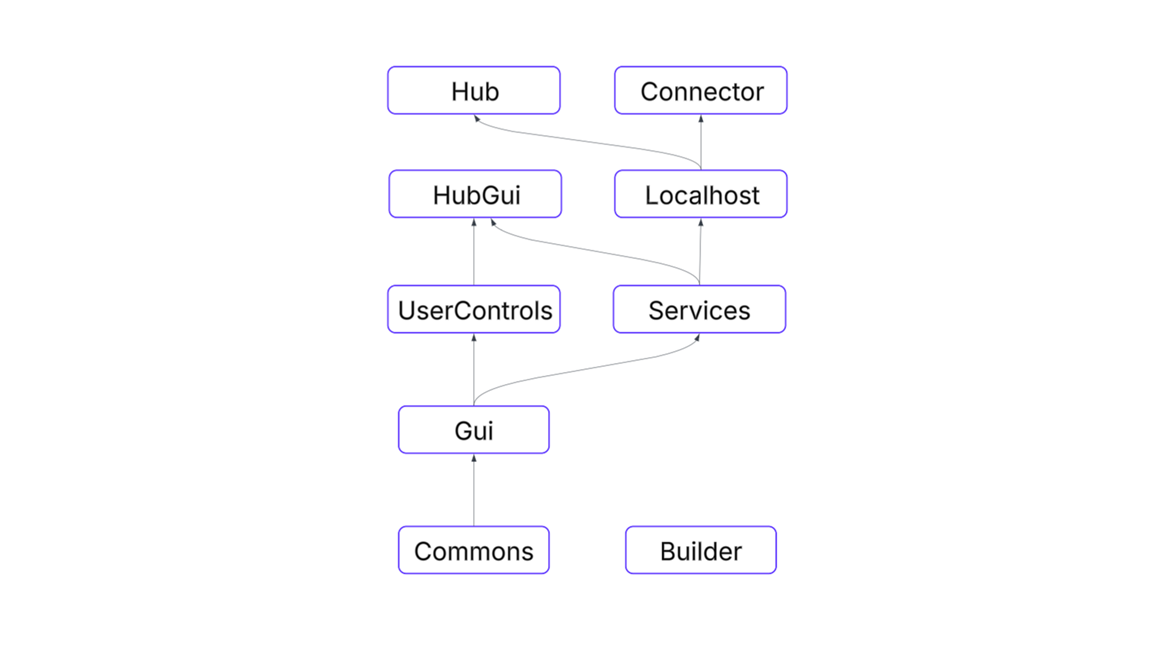
\includegraphics[width=\linewidth]{obrazky-figures/Structure.png}
    \caption{Architektura Oidis Frameworku -- hierarchie závislostí modulů.}
    \label{OidisModuly}
\end{figure}

Modul \texttt{Commons} představuje základní část celého frameworku a obsahuje společné komponenty, které jsou využívány napříč všemi ostatními moduly. Obsahuje zejména základní datové struktury, rozhraní, pomocné třídy a utility, jež umožňují budovat vyšší vrstvy systému. Součástí jsou také základní mechanismy validace dat, konvertory mezi různými datovými reprezentacemi, řetězcové utility, třídy pro práci s logováním a infrastruktura pro~psaní a spouštění jednotkových testů.

Modul \texttt{Gui} je zaměřen na grafické uživatelské rozhraní. Je postaven nad modulem \texttt{Commons} a rozšiřuje ho o prvky určené pro obsluhu grafické vrstvy. Obsahuje základní komponenty, které umožňují vykreslování uživatelského rozhraní, správu ikon, fontů a vizuálních prvků systému. Tento modul neřeší logiku aplikace ani nevytváří konkrétní GUI prvky. Stejně jako \texttt{Commons} představuje univerzalní modul, ale zaměřený na GUI vrstvu a~poskytuje technický základ, na kterém mohou vyšší vrstvy vytvářet vizuální prvky a~jednotné uživatelské prostředí.

Tyto dva moduly historicky vznikly pro práci s grafickými jádry prohlížečů a vykreslováním stránek. Hlavním cílem bylo zajistit jednotný vzhled webové stránky bez ohledu na~použitý prohlížeč, přičemž Oidis Framework fungoval jako polyfill, který vyrovnával rozdíly mezi různými jádry. V současnosti již tento problém není aktuální, nicméně moduly stále plní roli polyfillu z hlediska prostředí, ve kterém se kód vykonává -- zda v Node.js, nebo přímo v prohlížeči.

Modul \texttt{UserControls} rozšiřuje základy z předchozí vrstvy a obsahuje konkrétní, opakovaně použitelné prvky uživatelského rozhraní. Modul poskytuje sadu  hotových komponent, jako jsou tlačítka, textová pole, rozbalovací seznamy, dialogová okna nebo komponenty pro~nahrávání souborů. Tento modul tím umožňuje rychle sestavovat robustní grafické rozhraní bez nutnosti znovu implementovat základní funkce pro práci s vizuálními komponentami.

Modul \texttt{Hub} představuje ústřední logickou vrstvu celého frameworku. Zajišťuje koordinaci ostatních částí systému, řídí hlavní aplikační procesy a obsahuje implementaci klíčové obchodní logiky. Propojuje uživatelské rozhraní, servisní vrstvu i práci s daty do jednoho uceleného funkčního systému.

Modul \texttt{HubGui} poskytuje grafické rozhraní nad logickou vrstvou modulu \texttt{Hub}. Umožňuje vizualizovat data, ovládat aplikaci pomocí interaktivních prvků a poskytuje uživateli přehled o procesech probíhajících v jádru systému. Jedná se o prezentační vrstvu nad modulem \texttt{Hub} a rozšíření \texttt{UserControls}. Modul obsahuje vizuální komponenty pokrývající širokou škálu požadavků aplikace, ale neobsahuje žádnou obchodní logiku. Součástí modulu je také administrační rozhraní aplikace.

Modul \texttt{Services} pokrývá serverovou a servisní logiku. V rámci frameworku typicky obsahuje webové služby, REST API, rozhraní pro přístup k datům a integrační logiku pro~komunikaci s externími systémy nebo pro komunikaci frontendu s backendem. Tyto~služby mohou být provozovány na různých platformách a poskytovat funkcionalitu jak pro jádro systému, tak i pro uživatelské rozhraní.

Účelem modulu \texttt{Localhost} je poskytnout prostředí pro běh serveru. Obsahuje HTTP server a zajišťuje veškerou síťovou komunikaci, podobně jako Node.js framework Express.js. Kromě toho modul poskytuje funkcionalitu pro komunikaci s terminálem, práci se souborovým systémem a umožňuje spouštění příkazů a operace se soubory. Podporuje nasazení na různé platformy prostřednictvím předpřipravených konfiguračních profilů pro Windows, Linux, macOS i ARM zařízení.

Modul \texttt{Connector} je postaven nad modulem \texttt{Localhost} a slouží primárně jako základ pro tvorbu agentů -- samostatných procesů bez grafického 
rozhraní, které zajišťují sběr dat, komunikaci se vzdálenými zařízeními 
nebo integraci s externími systémy. Typickým scénářem je nasazení 
agenta na vzdáleném zařízení s komunikací přes reverzní tunel. \texttt{Connector} proto obsahuje dílčí obchodní logiku zaměřenou na tyto integrační a komunikační scénáře.

\texttt{Builder} zajišťuje sestavení, kompilaci a nasazení celého projektu. Závisí na modulech \texttt{Commons, Connector, Gui, Localhost} a \texttt{Services} a je spouštěn z příkazové řádky bez~grafického rozhraní. Jednou z charakteristických vlastností \texttt{Builderu} je, že sestavuje sám sebe -- předchozí verze musí být schopna zkompilovat verzi novou, podobně jako kompilátor GCC. Tento přístup přispívá k vysoké míře znovupoužitelnosti kódu v celém frameworku.

Ve většině případů, kdy je platforma Oidis využita pro vývoj, se jedná o aplikaci založenou na Node.js, která běží na serveru. Díky představeným modulům lze při vývoji využívat pouze nezbytnou funkcionalitu. Pro klasické webové aplikace je možné využít předpřipravené základní funkce pro správu uživatelů, správu aplikace, odesílání e-mailů, tisk či práci se soubory a stavět aplikaci nad moduly \texttt{Hub} a \texttt{HubGui}. V případě vývoje datových mostů lze jako základ použít modul \texttt{Localhost} a \texttt{Services}, pokud není nutné grafické rozhraní.

Obchodní logika aplikace je implementována v Node.js a běží nativně na dané platformě. Modul \texttt{Localhost} zajišťuje spuštění lokálního serveru a umožňuje nasledné nasazení aplikace na libovolný operační systém, včetně ARM zařízení, jako jsou Raspberry Pi nebo~IoT\footnote{IoT (Internet of Things) označuje síť fyzických zařízení vybavených senzory a připojením k internetu.} zařízení. Hybridní část aplikace, tedy vizuální rozhraní, je zpravidla řešena přístupem PWA tam, kde je to možné.

Aplikace se vyvíjejí v jazyce TypeScript objektově orientovaným způsobem. Většinou se~jedná o monolitickou architekturu, kde je přístup spíše podobný Windows Forms než~moderním frameworkům typu React nebo Vue, které využívají funkcionální programování.

\chapter{Relevance funkcionality vizuálních editorů pro Oidis Framework}
\label{Editory}
Oidis je společnost zabývající se vývojem webových aplikací na zakázku, se zaměřením na~aplikace pracující se specifickým hardwarem. Dodávané aplikace jsou postavené na platformě Oidis a Oidis Frameworku, který je orientován na využití webových technologií. Frontendová část aplikací je vyvíjena pomocí HTML, CSS a JavaScriptu, doplněných o jejich rozšíření, jako jsou TypeScript a Sass, a o knihovnu Bootstrap, která slouží jako zdroj předpřipravených komponent a stylů pro zajištění jednotného vzhledu aplikací a zjednodušení a urychlení implementačního procesu.

V současnosti je pro návrh UI komponent využíván grafický editor Bootstrap Studio, popsaný v sekci~\ref{BootstrapStudio}. Mezi dostupnými nástroji, které umožňují práci s knihovnou Bootstrap, byl vyhodnocen jako poskytující nejkomplexnější podporu této knihovny a jeho použití výrazně zrychluje proces implementace komponent. Ovšem funkcionalita poskytovaná Bootstrap Studio není postačující pro účely vývoje ve frameworku Oidis a cílem této~práce je zdokonalit způsob návrhu UI komponent při tvorbě aplikací postavených na~tomto frameworku.

Framework Oidis využívá komponentový přístup, kde každá komponenta má samostatný soubor i odpovídající návrh v Bootstrap Studiu. Tento způsob práce s grafickým editorem je vhodný pro vytváření nových komponent, ale následná synchronizace změn mezi editorem a kódem je zdlouhavá, protože každá úprava musí být provedena ručně na obou místech. Z těchto důvodů vznikl požadavek na vytvoření nového editoru, který zachová výhody Bootstrap Studia -- intuitivní vizuální návrh, snadné ovládání a práci s třídami a styly, ale~zároveň umožní úpravu komponent pouze na jednom místě.

Cílem této kapitoly je analyzovat vizuální editory webových aplikací a vyhodnotit, která~část jejich funkcionality je relevantní pro návrh grafického editoru v rámci platformy Oidis. V další sekci~\ref{FunkcionalitaBss} je provedena analýza funkcionality poskytované současně využívaným řešením Bootstrap Studio. Následně je v sekci~\ref{SoucasnyStav} popsán aktuální postup vývojářů při práci s Bootstrap Studio a jeho omezení. V sekci~\ref{Pozadavky} jsou poté představeny výsledné požadavky na nové řešení.

\section{Funkcionalita Bootstrap Studio}
\label{FunkcionalitaBss}
Bootstrap Studio představuje komplexní prostředí pro návrh webových rozhraní, jehož rozložení lze rozdělit do několika logických oblastí (obr.~\ref{BSS}). Každá z těchto zón podporuje specifickou část pracovního postupu při návrhu uživatelského rozhraní.

\begin{figure*}[h]\centering
  \centering
  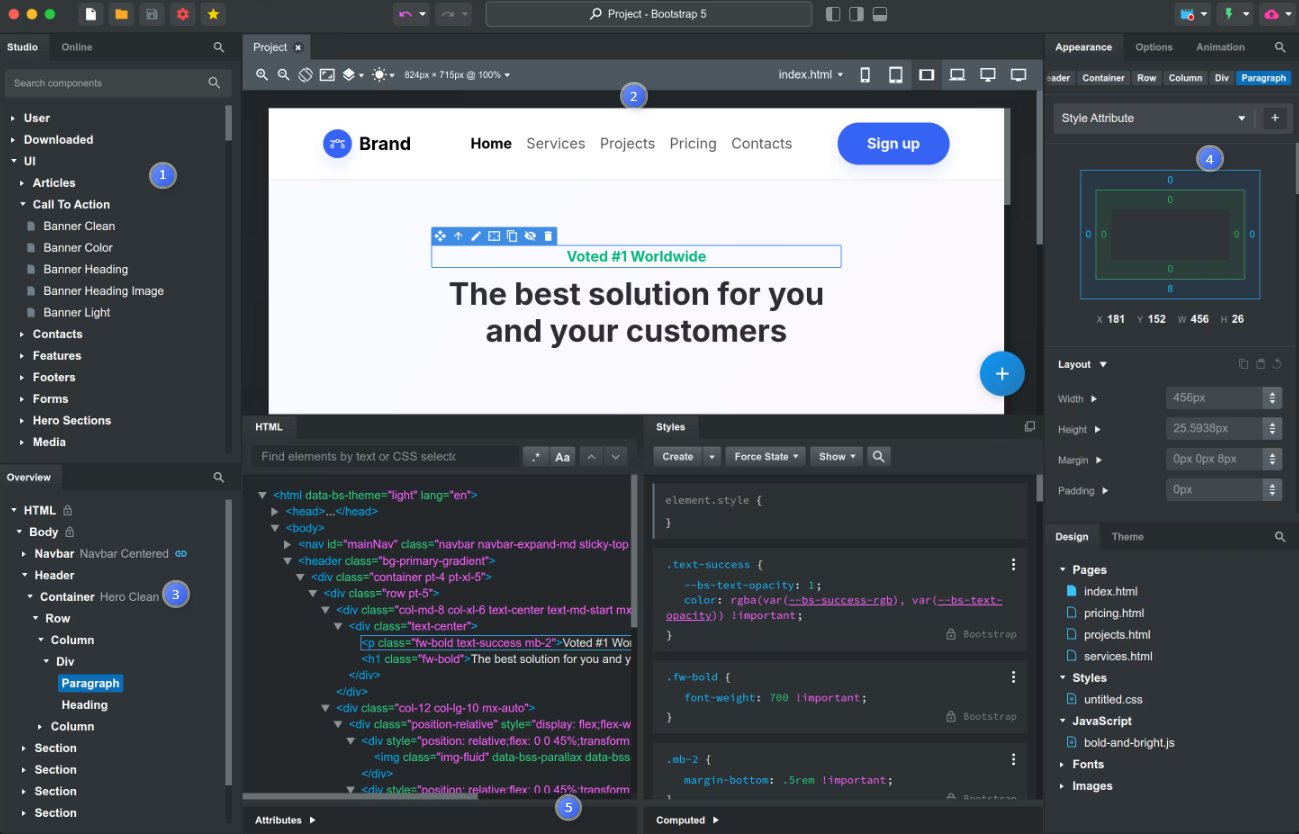
\includegraphics[width=\linewidth]{obrazky-figures/BSStudio.png}\hfill
  \caption{Náhled na vizuální editor Bootstrap Studio. Obrázek je převzat z webové stránky \url{https://bootstrapstudio.io}.}
  \label{BSS}
\end{figure*}

\textbf{Komponentní panel a knihovna komponent (zóna 1 obr. \ref{BSS})}. V levé části rozhraní se nachází komponentní panel, který slouží jako hlavní vstupní bod pro tvorbu návrhu. Bootstrap Studio poskytuje knihovnu vestavěných komponent odpovídajících standardním prvkům knihovny Bootstrap -- tlačítka, navigace, grid systém, formulářové prvky, multimédia, bloky rozložení prvků či modální okna. Tyto komponenty jsou organizovány do~kategorií a lze je filtrovat či vyhledávat. Komponentní panel představuje primární místo pro přidávání prvků do návrhu. Součástí panelu je také sekce User Components, která umožňuje vytvářet vlastní komponenty. Tyto komponenty lze exportovat ve formátu \texttt{.bscomp}, který interně obsahuje vlastní HTML, CSS i JavaScript a používat je v dalších projektech.

\textbf{Drag‑and‑drop vizuální návrh (zóna 2, 3 obr.~\ref{BSS})}. Hlavní pracovní plocha slouží jako vizuální editor, ve kterém uživatel metodou drag-and-drop sestavuje rozhraní. Komponenty z levého panelu lze přetáhnout na plátno, umístit do layoutu a dále upravovat jejich vizuální strukturu. Plocha podporuje běžné operace, jako je přesun prvků, jejich mazání, duplikace či reorganizace. Uživatel může rovněž přímo vizuálně měnit odstupy, velikosti prvků a další stylové vlastnosti, přičemž editor automaticky generuje odpovídající třídy knihovny Bootstrap nebo definice CSS stylů.

Tento přistup umožňuje vytvářet uživatelské rozhraní bez nutnosti manuální úpravy kódu. Je však třeba poznamenat, že ne všechny změny lze provést jednoznačně pomocí plátna -- zejména komplikované přesuny v hlubší struktuře nemusí být spolehlivé. Proto~je tato oblast rozšířena o stromovou strukturu dokumentu, která zobrazuje kompletní hierarchii komponent. Tento strom lépe zohledňuje strukturu výsledného HTML a umožňuje přesnější manipulaci s prvky, které nemusí být na plátně dobře uchopitelné.

\textbf{Aplikace stylu a nastavení komponent (zóna 4 obr. \ref{BSS})}. Pravá část rozhraní obsahuje panel pro konfiguraci stylů a vlastností komponent. Uživatel zde může měnit základní atributy prvků, nastavovat jejich parametry, pracovat s grid systémem nebo přidávat Bootstrap třídy. Všechny změny jsou následně automaticky přeneseny do kódu návrhu.

\textbf{Podpora editace kódu (zóna 5 obr. \ref{BSS})}. Bootstrap Studio umožňuje kdykoliv přejít z vizuálního návrhu do přímé editace kódu, především ale zaměřenou na úpravu stylů. Nabízí samostatná okna pro úpravu CSS (včetně SASS) a JavaScriptu. Tato okna obsahují vlastní sadu vizuálních ovládacích prvků. Uživatel tak může doplňovat atributy, nastavovat styly, přidávat třídy nebo měnit strukturu prvku jak textově, tak prostřednictvím doplňkových vizuálních akcí. Tento přístup je vhodný zejména v situacích, kdy vizuální editor nenabízí dostatečnou flexibilitu a je nutné některé detaily doladit přímo v kódu.

\section{Současný postup práce s Bootstrap Studio}
\label{SoucasnyStav}

Stávající i nové řešení je určeno vývojářům aplikací postavených na platformě Oidis. Primárně se jedná o vývojáře frontendové části projektů, kteří využívají vizuální editor pro~prvotní návrh komponent nebo jejich úpravy, případně o vývojáře, jejichž hlavním cílem není vývoj frontendu, ale kteří potřebují vytvořit jednoduchou komponentu pro zprovoznění minimální funkcionality nebo pro testování. Návrh nové komponenty v prostředí Bootstrap Studio začíná založením nového souboru, následuje sestavení struktury stránky a úprava vizuálního vzhledu komponenty. Přestože je tento postup funkční a relativně efektivní, v~praxi naráží na několik problémů vyplývajících z toho, že oba nástroje nebyly navrženy jako jediný systém.

Prvním z nich je skutečnost, že platforma Oidis využívá komponentový přístup, kde má každá komponenta samostatný soubor i odpovídající návrh v nástroji Bootstrap Studio, zatímco Bootstrap Studio předpokládá návrh celé aplikace v jednom souboru. Bootstrap Studio sice umožňuje přidat do jednoho návrhu více souborů či stránek, které by mohly sloužit k návrhu různých komponent, ale takový přístup představuje problém z hlediska verzování, protože při změně libovolné komponenty v projektu je upraven výsledný soubor Bootstrap Studia jako celek. Použití samostatných souborů pro návrh jednotlivých komponent řeší problém s verzováním, ale vzniká problém s využíváním globálně definovaných stylů. Bootstrap Studio umožňuje import CSS souborů, je však nutné tyto styly udržovat ručně pro každou komponentu zvlášť.

Dalším problémem týkajícím se samotného návrhu komponenty je skutečnost, že Bootstrap Studio sice umožňuje přidávat k prvkům libovolné atributy, včetně těch, které jsou nezbytné pro propojení s logikou komponent v Oidis Frameworku, jejich správa však není nijak specializovaná. Každý atribut je nutné zapisovat ručně -- včetně názvu, hodnoty i~potřebného prefixu, který se v Oidis používá pro propojení vizuálních prvků s aplikační logikou. Neexistuje zde možnost definice vyhrazeného pole nebo typu atributu, který by tuto práci usnadňoval. Přidávání identifikátorů pro logiku komponent (např. pro napojení na~data, události nebo API) je proto časově náročné a náchylné k chybám.

Po dokončení návrhu v Bootstrap Studio následuje ruční fáze: kompletní HTML kód vytvořený v grafickém editoru je třeba zkopírovat do kódového editoru v projektu Oidis. V~kódu se poté provádí napojení komponent na logiku. Postup práce s Bootstrap Studio je znázorněn na obrázku~\ref{BSSWorkflow}. Pro každý prvek, který má být programově ovládán nebo~sledován, je nutné vytvořit odpovídající proměnnou, inicializovat ji pomocí předpřipravené komponenty Oidis a propojit ji s konkrétním místem v HTML. Tento postup je nutný proto, že framework pracuje s originálními prvky Bootstrapu, ke kterým interně přidává funkcionalitu (například pro tlačítka, pole pro vstupy nebo interaktivní UI prvky).

Po dokončení této fáze je komponenta připravena k použití, avšak celý proces se výrazně komplikuje ve chvíli, kdy je nutné provést změnu designu. Výše uvedený postup je nutné aplikovat znovu, což znamená udělat úpravy v Bootstrap Studio, zkopírovat výsledný kód do kódového editoru, inicializovat nově přidané proměnné a sestavit projekt. Bootstrap Studio nabízí funkci náhledu v reálném čase, která slouží k rychlé vizuální kontrole, ale~tato možnost v kontextu Oidis Frameworku často neodpovídá skutečnému výsledku. V~Oidis se~stránka skládá z více samostatných komponent, z nichž každá vzniká odděleně. Kvůli~tomu náhled v Bootstrap Studio zobrazuje komponentu izolovaně -- bez rámce celé stránky, a výsledný vzhled může být odlišný. Testování úprav je nutné provádět až za běhu aplikace, a jakmile se objeví chyba nebo potřeba další úpravy, celý cyklus se opakuje.

Zkušenější vývojáři tento proces často urychlují tím, že změny provádějí rovnou v kódu bez použití vizuální editace Bootstrap Studio. Tím se sice eliminuje část zdlouhavé práce, ale~zároveň vzniká nový problém: návrh v Bootstrap Studio se přestane shodovat se skutečným stavem komponenty v projektu. Proto je potřeba komponentu dále vizuálně upravit, ručně přenést všechny změny z kódu zpět do Bootstrap Studio, aby byl návrh aktuální a~mohl sloužit jako podklad pro další úpravy. Paralelní aktualizace kódu i vizuálního návrhu je časově náročná, snadno vede k nesrovnalostem a představuje jeden z nejvýznamnějších nedostatků současného pracovního postupu. 

\begin{figure*}[h]\centering
  \centering
  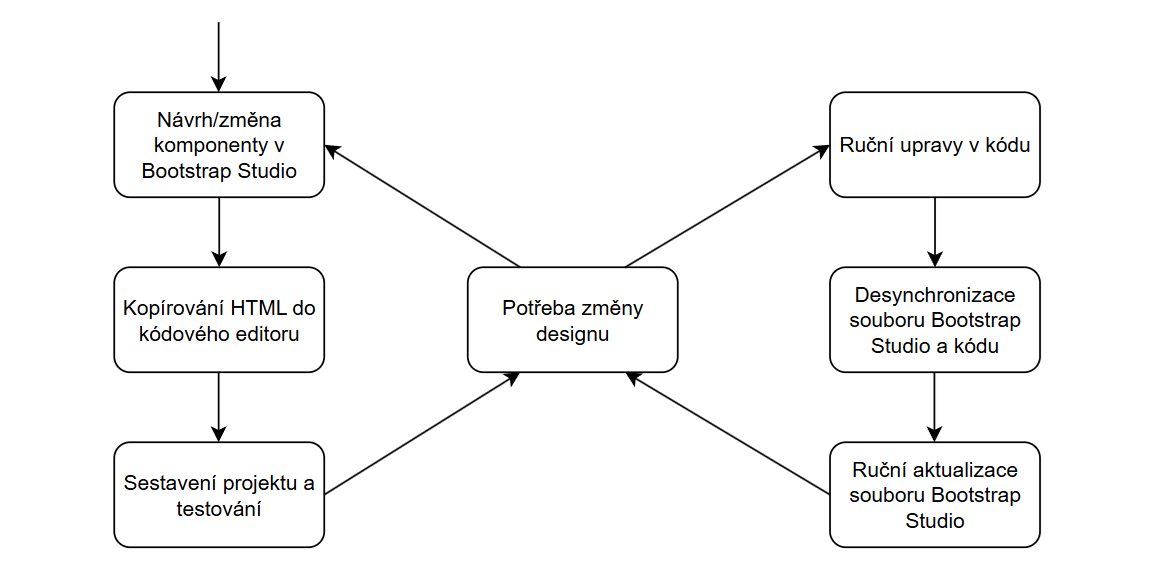
\includegraphics[width=\linewidth]{obrazky-figures/Workflow.png}\hfill
  \caption{Postup práce s Bootstrap Studio při vývoji komponent 
    pro použiti v projektu postaveném na frameworku Oidis.}
  \label{BSSWorkflow}
\end{figure*}

Dalším nedostatkem je práce se styly, které jsou v projektu Oidis obvykle umístěny v souborech SASS a nejsou přímo připojeny k jednotlivým HTML prvkům. Bootstrap Studio sice umí pracovat se soubory SASS, ale znovu se zde projevuje rozdílný přístup k~návrhu komponent. V aplikaci existuje sada komponent, z nichž každá může, ale nemusí mít vlastní samostatný soubor SASS. Pokud nejde o rozsáhlejší komponentu, mohou být její styly součástí globálního souboru SASS konkrétní stránky, na které se komponenta používá. Protože je pro každou komponentu vytvářen samostatný soubor v Bootstrap Studio, je nutné při každém návrhu ručně kopírovat odpovídající SASS soubory, aby vizuální náhled co nejlépe odpovídal reálnému vzhledu. Tím se workflow dále prodlužuje a vyžaduje neustálé manuální aktualizace stylů.

\section{Požadavky Oidis Studio}
\label{Pozadavky}
Jak vyplývá ze sekce~\ref{SoucasnyStav}, aktuální řešení vykazuje řadu nedostatků, které jsou způsobeny tím, že Bootstrap Studio nebylo navrženo primárně pro práci s platformou Oidis a zároveň uplatňuje odlišný přístup k návrhu aplikací. Předpokládá návrh celé aplikace v jednom souboru se zaměřením na statické stránky, u nichž se nepředpokládají časté úpravy již~vytvořených návrhů. Přesto nabízí i řadu výhod, které usnadňují práci a urychlují návrh komponent.

Nová aplikace by na základě analýzy nedostatků současného řešení měla zachovat základní funkcionalitu a rozšířit ji o nové funkce, které by uvedené nedostatky odstranily. Základní požadavky na Oidis Studio jsou definovány následovně:

\begin{itemize}
\item Drag-and-drop editace HTML struktury komponenty nebo stránky.
\item Seznam dostupných základních komponent, pomocí nichž je možné sestavit výsledný návrh, včetně základních komponent knihovny Bootstrap.
\item Možnost nastavení tříd a atributů pro komponenty, zejména se zaměřením na knihovnu Bootstrap.
\item Možnost zpracování existujícího souboru, který obsahuje HTML strukturu komponenty, a jeho zobrazení ve vizuálním editoru s možností úprav.
\item Automatické načtení konfiguračních souborů projektu obsahujících metadata dostupných komponent frameworku Oidis.
\item Správa atributu \texttt{data-oidis-bind} s možností výběru dostupného typu komponenty frameworku, včetně automatického generování odpovídajících importů ve výsledném souboru.
\item Generování kódu do TypeScript třídy ve formátu použitelném pro další práci ve frameworku Oidis.
\end{itemize}

Mezi doporučené požadavky na funkcionalitu výsledného grafického editoru patří možnost nastavování inline stylů pomocí vizuálních prvků, responzivní náhled komponenty pro~různé velikosti obrazovky v souladu s breakpointy knihovny Bootstrap a přímá editace HTML/CSS kódu.

\chapter{Pracovní postup aplikace a návrh uživatelského rozhraní}
\label{Navrh}

Tato kapitola je zaměřena na popis uživatelského postupu při práci s aplikací Oidis Studio v propojení s dalšími nástroji platformy Oidis. Součástí kapitoly je rovněž návrh uživatelského rozhraní aplikace a popis mechanismů, pomocí nichž bude zajištěno její zapojení do~vývojového procesu.

\section{Pracovní postup uživatele}
Jak bylo uvedeno v předchozích kapitolách, cílovou skupinou uživatelů Oidis Studio jsou především vývojáři zodpovědní za frontendovou část aplikací. Tito uživatelé se primárně zaměřují na tvorbu webových stránek nebo UI komponent od začátku, případně na jejich úpravy v reakci na změny designu. Pro tuto skupinu má použití Oidis Studio oproti současnému řešení přinést zásadní výhodu zejména ve vylepšení generování výsledného kódu komponenty nebo stránky, který by obsahoval definované proměnné pro propojení uživatelského rozhraní s aplikační logikou. Zároveň by použití Oidis Studio mělo vést k výraznému zjednodušení práce při změnách designu, jelikož bude eliminována nutnost dvojí údržby kódu aplikace a návrhu v nástroji Bootstrap Studio. Vývojář bude schopen nahrát existující komponentu přímo do Oidis Studio a provádět její úpravy, případně se pro drobné změny rozhodnout pracovat přímo v kódu bez využití vizuálního editoru. Výsledný stav komponenty však bude v obou případech korektní a připravený pro další vizuální úpravy. 

Další skupinou uživatelů jsou programátoři, jejichž hlavním zaměřením není frontendový vývoj, přesto však potřebují vytvářet jednodušší uživatelské komponenty. Tito uživatelé mohou využít výhod vizuálního sestavování výsledného kódu komponenty bez nutnosti hlubších znalostí frontendových technologií.

Workflow práce s Oidis Studio je navržen tak, aby podporoval dva základní scénáře: vytvoření nové komponenty a úpravu již existující komponenty. Aplikace vždy pracuje s existujícím souborem -- v případě úpravy stávající komponenty jej zpracuje, extrahuje HTML obsah a zobrazí jej na editační ploše, v případě nové komponenty se předpokládá, že vývojář založí prázdný soubor na odpovídajícím místě v projektu a otevře jej v editoru, který následně vygeneruje požadovaný kód. Z hlediska interakce uživatele probíhají oba scénáře téměř totožně a liší se pouze tímto vstupním krokem. Postup práce je následující:

\begin{enumerate}
    \item {Import existujícího souboru v jazyce TypeScript -- soubor obsahuje existující HTML strukturu komponenty, nebo je prázdný v případě vytváření nové komponenty. Soubory určené pro práci v editoru by měly obsahovat vyhrazené bloky označené komentáři, do nichž je při exportu injektován generovaný HTML obsah, deklarace proměnných, jejich inicializace a importy. Import souboru bude probíhat po spuštění aplikace, kde uživatel bude vyzván k zadání cesty k cílovému souboru. Rozpoznání aktuálního souboru, se kterým aplikace pracuje, bude pravděpodobně realizováno podle parametrů v URL adrese stránky.}
    \item {Na základě umístění otevřeného souboru Oidis Studio automaticky prohledá katalog projektu a načte odpovídající konfigurační soubory s metadaty dostupných komponent frameworku (viz. sekci~\ref{metadata}).}
    \item {Úprava komponenty v grafickém editoru:
    \begin{itemize}
        \item {Přidání nových prvků z katalogu komponent.}
        \item {Nastavení tříd knihovny Bootstrap nebo úprava inline stylů jednotlivých prvků.}
        \item {Přidání dalších atributů, včetně atributu \texttt{data-oidis-bind} pro propojení s aplikační logikou frameworku.}
    \end{itemize}}
    \item {Export vygenerovaného kódu jedním z následujících způsobů:
        \begin{itemize}
            \item {Vygenerování a uložení kompletního souboru v jazyce TypeScript.}
            \item {Uložení změn do importovaného souboru nahrazením sekce s HTML obsahem komponenty, inicializací proměnných definovaných v grafickém editoru pro propojení s frameworkem a vytvořením odpovídajících importů podle načteného konfiguračního souboru.}
            \item {Zkopírování pouze HTML obsahu v případě, že není nutné generovat celý soubor v jazyce TypeScript.}
        \end{itemize}
    }
\end{enumerate}

\section{Návrh uživatelského rozhraní}

V sekci~\ref{Pozadavky} byly vymezeny základní požadavky na funkcionalitu, které by měla aplikace obsahovat a které je možné převzít z nástroje Bootstrap Studio. Níže je představen návrh uživatelského rozhraní aplikace (obr.~\ref{Design}).

\begin{figure*}[h]\centering
  \centering
  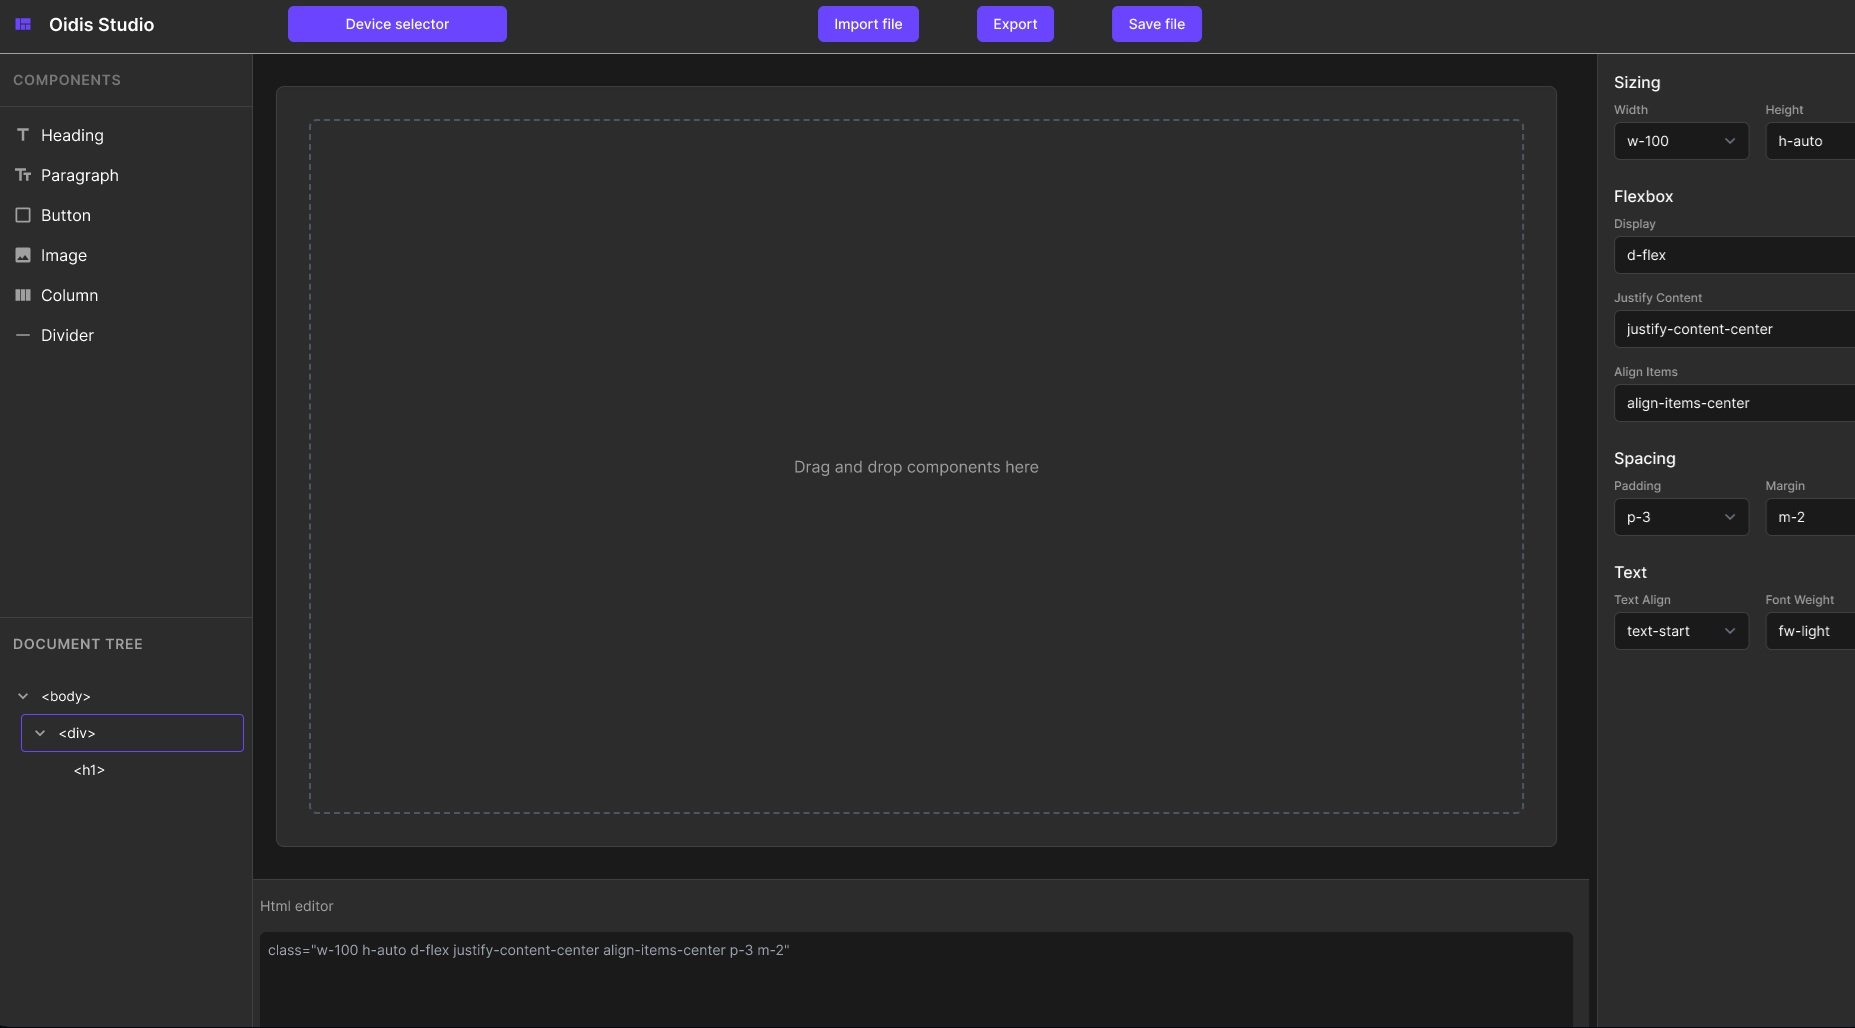
\includegraphics[width=\linewidth]{obrazky-figures/Design.jpg}\hfill
  \caption{Návrh uživatelského rozhraní Oidis Studio. Levá část obsahuje katalog komponent a strom HTML prvků. Centrální část tvoří editační plocha s náhledem komponenty včetně ovládacích nástrojů a editor kódu 
s aktuálním stavem výsledné HTML struktury. Pravá část obsahuje panel vlastností vybraného prvku a jeho stylování.}
  \label{Design}
\end{figure*}

V levé části rozhraní se nachází katalog komponent, ve kterém jsou umístěny všechny dostupné UI prvky uspořádané podle jednotlivých kategorií. Katalog obsahuje standardní komponenty knihovny Bootstrap a uživatelské komponenty generované na základě načtených souborů metadat. Tyto uživatelské komponenty odpovídají konkrétnímu projektu, se~kterým uživatel aktuálně pracuje, a umožňují tak přímé využití komponent definovaných v rámci daného projektu při návrhu 
uživatelského rozhraní. 

Hlavní část rozhraní tvoří centrální pracovní plocha určená pro editaci návrhu komponenty. Do této oblasti je možné přetahovat nové UI prvky z levého panelu nebo měnit uspořádání již existujících prvků. Tato oblast slouží především jako náhled výsledné podoby komponenty a umožňuje interaktivní práci s prvky, jejich výběr a následné nastavování vlastností. Doplňkem centrální pracovní plochy je strom HTML prvků, ve kterém je možné přesouvat již existující elementy. Účelem této části je umožnit provádění operací, které nelze realizovat přímo v centrální pracovní oblasti, a zároveň poskytnout přehled o struktuře výsledného DOM stromu. Ve spodní části oblasti se nachází editor kódu zobrazující aktuální podobu kódu, který bude obsažen ve výsledném exportovaném souboru.

V pravé části aplikace se nachází oblast určená pro manipulaci s vlastnostmi jednotlivých prvků. Po výběru elementu ve stromu nebo ve vizuálním editoru se zobrazí dostupné vlastnosti daného elementu, které lze upravovat pomocí grafických ovládacích prvků. Zvolené nastavení je následně propagováno do kódu ve formě Bootstrap tříd nebo vestavěných stylů, a jeho efekt je okamžitě viditelný v editační oblasti.

V horní části aplikace se nachází hlavička obsahující sadu doplňkových nástrojů, jako~je přepínání rozměrů pracovní plochy pro náhled v různých velikostech obrazovky, import a~export souboru komponenty nebo další pomocné funkce.

Celkový design aplikace je inspirován nástrojem Bootstrap Studio, jehož rozhraní odpovídá požadavkům kladeným na podobné typy editorů a poskytuje přehledné a komfortní pracovní prostředí. Dalším důvodem pro zvolenou podobu rozhraní je skutečnost, že Bootstrap Studio je v současnosti využíváno při vývoji aplikací postavených na frameworku Oidis, a jeho rozvržení i způsob práce jsou vývojářům již dobře známé. Tento přístup usnadňuje přechod na nový nástroj.

Funkcionalita je v některých částech záměrně zjednodušena oproti Bootstrap Studio, a~to~z~důvodu nízké míry jejího využití v rámci běžného vývoje nebo s ohledem na prioritní implementaci základních mechanismů aplikace. Tyto funkcionality budou postupně rozšiřovány v budoucích verzích. Mezi plánovaná rozšíření patří například vyhledávání v katalogu komponent, podpora různých rozměrů pracovní plochy, odpovídajících různým typům zařízení, nebo možnost importu barevné palety a načtení SASS a CSS souborů projektu.

\section{Propojeni s frameworkem Oidis}
\label{metadata}
Jak bylo uvedeno v sekci~\ref{ArchitekturaOidisFrameworku}, většina projektů postavených na frameworku Oidis využívá třídy určené pro práci s komponentami knihovny Bootstrap. Při použití vizuálních prvků, ke kterým je nutné doplnit aplikační logiku, jsou tyto třídy propojeny s konkrétními prvky prostřednictvím atributu \texttt{data-oidis-bind}. Aby bylo možné tento proces v Oidis Studio automatizovat, je nezbytné mít k dispozici přehled tříd odpovídajících komponent knihovny Bootstrap a také dalších komponent dostupných v rámci konkrétního projektu.

Pro tyto účely by měly být v projektu definovány konfigurační soubory, které Oidis Studio načte a na jejich základě rozšíří katalog dostupných komponent a automatizuje generování výsledného kódu. Navrhované řešení předpokládá dva typy těchto souborů lišící se účelem a obsahem.

První typ by popisoval komponenty modulu \texttt{io-oidis-usercontrols}, tedy třídy frameworku Oidis zajišťující práci se standardními prvky knihovny Bootstrap. Každý záznam by měl obsahovat seznam názvů Bootstrap elementů, které daná třída obsluhuje, název třídy a cestu k její implementaci. Příklad struktury takového záznamu je uveden ve výpisu~\ref{lst:bootstrapconfig}.

\begin{lstlisting}[
  float=h,
  caption={Příklad záznamu konfiguracního souboru pro třidu odpovídající komponentě knihovny Bootstrap.},
  label={lst:bootstrapconfig}
]
"components": [
  {
    "name": ["button"],
    "className": "Button",
    "path": "@io-oidis-usercontrols/.../Button.js"
  }
]
\end{lstlisting}

Druhý typ by popisoval komponenty specifické pro konkrétní projekt, tedy vlastní třídy vytvořené vývojářem, které nejsou součástí standardních modulů frameworku. Oproti předchozímu formátu by obsahoval navíc pole definující HTML strukturu sloužící jako placeholder komponenty v editační ploše. Tato struktura by představovala vizuální reprezentaci komponenty v editoru, přičemž ve výsledném exportovaném souboru by byla nahrazena správnou instancí třídy. Příklad struktury takového záznamu je uveden ve výpisu~\ref{lst:projconfig}.

\begin{lstlisting}[
  float=h,
  caption={Příklad záznamu konfiguracního souboru pro třidu specifickou pro projekt.},
  label={lst:projconfig},
  breaklines=true,
  breakatwhitespace=true
]
"components": [
  {
    "name": "mainComponent",
    "label": "Main Component",
    "className": "MainComponent",
    "path": "@io-oidis-studio-gui/
    Io/Oidis/Studio/Gui/Panels/MainComponent.js",
    "category": "Project components",
    "htmlPattern": "<div><span>MainComponent</span></div>"
  }
]
\end{lstlisting}

\chapter{Implementace}
\label{Implementace}

Tato kapitola se zabývá implementací grafického editoru Oidis Studio. Zaměřuje se~na~zohlednění architektury aplikace, popis použitých knihoven a konkrétních částí projektu, v~nichž~byly tyto knihovny využity, včetně způsobu jejich použití. Věnuje se řešením použitým při tvorbě dílčích bloků editoru, vizuální stránce aplikace a práci se soubory.

\section{Architektura aplikace}

Implementace grafického editoru je postavena na frameworku Oidis. Aplikace je navržena jako lokálně provozované řešení, které je uživateli zpřístupněno prostřednictvím webového prohlížeče. Toto řešení umožňuje využít výhod webového prostředí při práci s webovými komponentami, což zajišťuje lepší synchronizaci mezi navrhovanou komponentou a jejím reálným použitím. Zároveň využití frameworku Oidis umožňuje práci se souborovým systémem a rozšiřuje funkcionalitu o možnosti, které nejsou při běžném webovém vývoji standardně dostupné. Možnosti webového prohlížeče jsou přitom dostatečné pro provoz aplikace v podobě lokálního řešení a pro zajištění bezpečnosti při práci se soubory na zařízení uživatele.

Celé řešení je rozděleno do dvou repozitářů, obdobně jako u standardních projektů využívajících Oidis Framework. První repozitář zajišťuje aplikační logiku a konfiguraci projektu. Obsahuje funkcionalitu související se zpracováním souborů, včetně jejich vyhledávání, načítání, částečného zpracování a ukládání na disk. Druhý repozitář obsahuje klientskou část aplikace, totiž uživatelské rozhraní editoru, zpracování vstupů uživatele a komunikaci s~aplikační vrstvou. Tento repozitář je k hlavní části projektu připojen jako závislost.

Základem aplikace jsou moduly \texttt{Localhost} a \texttt{Services} frameworku, na kterých je celé řešení postaveno. Podle popisu v sekci~\ref{ArchitekturaOidisFrameworku} modul \texttt{Localhost} tvoří základ běhového prostředí aplikace. Zajišťuje spuštění HTTP serveru nad platformou Node.js a nabízí také~přístup k souborovému systému. Díky tomu je možné realizovat nejen obsluhu klientské části aplikace, ale také veškeré operace související se správou souborů, jejich načítáním, ukládáním a transformací. Modul \texttt{Localhost} tak fakticky nahrazuje klasickou serverovou infrastrukturu a umožňuje provoz aplikace plně lokálně, přičemž zachovává stejné principy jako u standardních webových aplikací.

Modul \texttt{Services} představuje aplikační vrstvu zajišťující zapouzdření jednotlivých funkčních celků systému. Odpovídá za propojení modulů a umožňuje jejich vzájemnou komunikaci.

Popsaná architektura umožňuje oddělit uživatelské rozhraní editoru od logiky práce se~soubory a zároveň zachovat přehlednou strukturu projektu. Toto oddělení je zároveň nezbytné, protože frontendová část sama o sobě nemůže zajistit využití funkcionality práce se soubory v rozsahu požadovaném touto aplikací. Zvolený přístup tak umožňuje tuto funkcionalitu realizovat prostřednictvím odpovídající aplikační vrstvy

\section{Implementace jednotlivých bloků editoru}
\label{GrapeJs}

Klientská část aplikace je postavena na knihovně GrapesJS\footnote{https://grapesjs.com/docs}, která slouží jako základ pro~vizuální návrh uživatelského rozhraní. Tato knihovna byla zvolena především díky podpoře práce metodou drag-and-drop a svému internímu zpracování obsahu vytvořeného návrhu prostřednictvím vlastního komponentového modelu, v němž je každý prvek stránky (např.~\texttt{div}, obrázek nebo tlačítko) reprezentován jako samostatná komponenta s definovanými vlastnostmi, strukturou a chováním. Tento model umožňuje nejen vizuální manipulaci s prvky, ale také jejich jednoznačnou reprezentaci, která je následně serializována do výstupního HTML kódu. Tato vlastnost je klíčová pro generování kódu a jeho další zpracování v rámci platformy. Zároveň je možné nabízenou funkcionalitu knihovny snadno rozšiřovat nebo upravovat.

\subsection{Editační plocha a stromová reprezentace}
Editační plocha a stromová reprezentace DOM struktury představují základní prvky uživatelského rozhraní editoru. Obě části jsou převzaty z knihovny GrapesJS a tvoří jádro interakce uživatele s aplikací. Editační plocha umožňuje vytváření elementů jejich přetažením z nabídky komponent a následnou manipulaci s těmito prvky přímo v rámci plochy. Uživatel může měnit jejich pozici, vnoření i hierarchii pomocí drag-and-drop operací. Veškeré změny se okamžitě promítají do stromové struktury a naopak. Stromová reprezentace rovněž umožňuje manipulaci s hierarchií prvků, což poskytuje alternativní způsob práce s~prvky. Obě části jsou vzájemně synchronizovány, přičemž tato synchronizace je zajištěna interní reprezentací dokumentu v knihovně GrapesJS.

\subsection{Katalog komponent a definice typů}
Na editační plochu přímo navazuje katalog komponent, který představuje zdroj prvků dostupných pro návrh uživatelského rozhraní.
V rámci této práce je katalog založen především na prvcích knihovny Bootstrap, která je využívána jako základní stavební prvek jak~pro~návrh rozhraní v editoru, tak pro vizuální podobu samotné aplikace. Tento přístup vychází z~toho, že Bootstrap je standardně používán při vývoji aplikací na frameworku Oidis, a~proto~jeho komponenty tvoří přirozený základ i pro návrhové prostředí editoru.

Katalog komponent je implementován pomocí vestavěného správce bloků knihovny GrapesJS, který~umožňuje vkládání předdefinovaných komponent do editoru. Protože výchozí sada komponent GrapesJS neodpovídá požadavkům této aplikace, zejména s ohledem na~použiti prvků knihovny Bootstrap, byly definovány vlastní typy komponent. Každý~typ komponenty obsahuje definici HTML struktury, dostupných vlastností a pravidel pro její rozpoznání v rámci dokumentu. Tím je zajištěno, že jednotlivé prvky lze nejen vizuálně upravovat, ale také jednoznačně interpretovat při generování výsledného kódu. Příklad takové definice typu komponenty je ve výpisu~\ref{lst:createtype}.

V rámci integrace s Oidis Frameworkem byl nejprve vytvořen základní typ komponenty, který obsahuje společné vlastnosti sdílené napříč všemi prvky. Tento základ byl následně rozšiřován o specifické vlastnosti a chování pro jednotlivé typy komponent. Na tomto principu byly vytvořeny komponenty odpovídající standardním HTML prvkům, prvkům knihovny Bootstrap a také specifickým prvkům definovaným v rámci Oidis Frameworku.

\subsection{Nastavení vlastností komponent}
Efektivní práce uživatele vyžaduje možnost nastavovat vlastnosti jednotlivých komponent. K tomuto účelu jsou využity bloky knihovny GrapesJS určené pro správu stylů a atributů. Při výběru konkrétního prvku editor automaticky načte parametry definované pro daný typ komponenty a zobrazí je v odpovídajících konfiguračních blocích.

Definice jednotlivých parametrů probíhá při návrhu typů komponent a je pevně svázána s konkrétní komponentou. Každý typ tak určuje, jaké vlastnosti lze u daného prvku nastavovat, jakým způsobem jsou reprezentovány v uživatelském rozhraní a jak se promítají do~výsledného HTML. Byla implementována vlastní vizuální reprezentace jednotlivých parametrů, byly upraveny existující komponenty pro zadávání hodnot uživatelem. Součástí této úpravy bylo také definování obslužných funkcí reagujících na změny hodnot, které~zajišťují jejich správnou propagaci do atributů nebo stylů příslušné komponenty v editoru.

Definice základního typu komponenty, který slouží jako výchozí pro vytváření dalších specifických typů, obsahuje obecné vlastnosti dostupné pro všechny elementy, přičemž důraz je kladen zejména na podporu principů knihovny Bootstrap, práci s třídami a základními stylovacími pravidly. Každý další typ vytvořený na základě tohoto typu jej rozšiřuje o specifická nastavení vázaná na konkrétní komponentu, která reflektují její charakter a omezení. Součástí implementace je také podpora responzivního nastavení atributů a stylů. Uživatel může definovat odlišné hodnoty pro různé velikosti zobrazovacího okna v souladu se~specifikací Bootstrapu.

\subsection{Vizuální podoba aplikace}
Vizuální podoba aplikace byla původně navržena podle rozvržení nástroje Bootstrap Studio a implementována podle návrhu uživatelského rozhraní představeného v sekci~\ref{Navrh}. Výsledná podoba aplikace se však od původního návrhu v některých detailech liší. Hlavní příčinou je využití knihovny GrapesJS, jejíž bloky a ovládací prvky přinášejí ve výchozím stavu vlastní vizuální styl. Při implementaci byl kladen důraz především na funkčnost a správné chování jednotlivých částí aplikace, zatímco úplné sjednocení vizuální stránky bylo ponecháno jako~úkol pro další fáze vývoje. Aktuální stav aplikace je zachycen na sadě obrázků v příloze~\ref{screen}.

\subsection{Konfigurace knihovny Bootstrap}
Knihovna Bootstrap je v této práci využívána jak pro vizuální vzhled samotné aplikace, tak pro vizuální ověření vytvářeného návrhu na editační ploše. Knihovnu je možné využívat i v její výchozí konfiguraci. V případě potřeby přizpůsobení vizuálního stylu nebo chování komponent však Bootstrap nabízí mechanismy umožňující jeho další konfiguraci prostřednictvím samostatného projektu založeného na SASS, což je přístup využívaný ve většině projektů na frameworku Oidis. V něm lze upravovat klíčové proměnné určující barevné schéma, typografii, velikosti prvků nebo breakpointy. Po kompilaci vznikne minimalizovaný CSS soubor, který lze zahrnout do cílové aplikace. Tento přístup umožňuje přizpůsobit vizuální podobu knihovny konkrétním požadavkům bez nutnosti přepisování stylů v cílové aplikaci.

V implementovaném řešení byla tímto způsobem vytvořena vlastní 
konfigurace Bootstrapu reflektující vizuální styl platformy Oidis, zejména z pohledu barevného schématu. Takto vygenerované styly jsou použity napříč celou aplikací a určují vzhled komponent Bootstrap použitých při vývoji.

Kromě globální konfigurace existuje mechanismus umožňující připojení odlišné konfigurace Bootstrapu přímo k editační ploše GrapesJS. Vedle stylů samotné aplikace tak může být dynamicky načten další konfigurační soubor, který ovlivňuje pouze vykreslování návrhu v editoru. Tento princip otevírá prostor pro budoucí rozšíření, kdy bude aplikace schopna automaticky načítat konfiguraci Bootstrapu konkrétního projektu, se kterým uživatel pracuje, a zobrazovat návrh přesně v té podobě, v jaké se objeví ve výsledné aplikaci.

Připojení Bootstrapu přímo k editační ploše má zásadní význam pro 
přesnost návrhu. Při změně vlastnosti komponenty v panelu nastavení jsou komponentám přiřazovány odpovídající Bootstrap třídy. Knihovna Bootstrap následně automaticky aplikuje příslušné styly a vizuální změna se okamžitě projeví v náhledu bez dodatečného zpracování. Pro úplnost je třeba poznamenat, že některé komponenty Bootstrap s interaktivním chováním (například modální okna či rozbalovací seznamy) vyžadují k plné funkčnosti vlastní JavaScriptový kód knihovny. V náhledu editoru je proto zobrazen pouze jejich vizuální stav, zatímco interaktivní logika je zprovozněna až ve výsledné aplikaci.

\section{Propojení s frameworkem Oidis}
\label{Propojeni}

Hlavním cílem aplikace není jen generování HTML struktury vytvořené ve vizuálním editoru, ale produkce kompletního výstupního souboru v jazyce TypeScript, který odpovídá konvencím frameworku Oidis a je přímo použitelný v cílovém projektu. V následujících sekcích je popsána práce se vstupním souborem, struktura a význam konfiguračních souborů a proces exportu, při kterém je na základě vytvořeného návrhu generován výsledný kód.

\subsection{Formát cílového souboru}

Komponenty ve frameworku Oidis jsou implementovány jako třídy dědící ze základní třídy \texttt{BasePanel}. Třída komponenty typicky obsahuje deklarace proměnných odpovídajících interaktivním prvkům uživatelského rozhraní, jejich inicializaci 
v konstruktoru a metodu vracející HTML šablonu, která tyto prvky propojuje s vizuální podobou komponenty.

Aby editor mohl s těmito soubory pracovat, byly do nich zavedeny vyhrazené bloky ohraničené komentáři. Tyto bloky vymezují oblasti, jejichž obsah je spravován editorem a~při~uložení komponenty je v nich umístěn nově vygenerovaný kód. Zbytek souboru, tedy~obchodní logika, obsluha událostí nebo doplňkové metody třídy, leží mimo vyznačené oblasti a editor jej nijak neupravuje. Díky tomuto rozdělení může tentýž soubor sloužit jako vstup i výstup editoru. Otevřením souboru se obsah bloku obsahující HTML strukturu načte a předá editační ploše ke zpracování a po uložení změn se přepíše pouze obsah vyhrazených bloků. Příklad souboru je ve výpisu~\ref{lst:file}

Aplikace však může pracovat i se soubory, které neobsahují explicitně vymezené bloky. Tyto soubory musí být validní třídou v jazyce TypeScript a zároveň by měly odpovídat konvencím zavedeným ve frameworku Oidis pro implementaci komponent. Při importu takového souboru je na základě klíčových slov a struktury kódu možné rozpoznat jednotlivé části komponenty a uchovat si informaci o jejich umístění. Při následném exportu jsou do~souboru doplněny vyhrazené bloky a do nich vložen generovaný obsah, zatímco ostatní části zdrojového kódu zůstávají beze změny.

\subsection{Konfigurační soubory projektu}

Aby editor dokázal generovat odpovídající importy a typy proměnných, potřebuje znát mapování mezi vizuálními prvky a třídami frameworku, které~obsluhují jejich logiku. Tato~znalost je předávána prostřednictvím dvou typů konfiguračních souborů, které byly představeny v návrhové části práce (viz. sekce~\ref{metadata}).

V rámci této práce byly konfigurační soubory vytvářeny ručně za účelem ověření jejich struktury a funkce. Automatizované generování těchto souborů přímo nástroji platformy Oidis je plánováno jako navazující krok po integraci řešení do platformy. Byly vytvořeny dva soubory -- první popisuje modul \texttt{io-oidis-usercontrols}, který ve svém základu odpovídá za práci s prvky knihovny Bootstrap, a druhý modeluje situaci, kdy jsou v rámci cílového projektu definovány vlastní komponenty.

Při načtení souboru určeného pro práci ve vizuálním editoru dochází na základě jeho umístění k prohledání projektového katalogu nástrojem Oidis Studio a k automatickému načtení odpovídajících konfiguračních souborů. V případě konfiguračního souboru modulu \texttt{io-oidis-usercontrols}, který zajišťuje práci s prvky knihovny Bootstrap již definovanými ve vizuálním editoru, je interní model těchto komponent rozšířen o dodatečné informace z~konfiguračního souboru. Každá komponenta tak obsahuje nejen svou vizuální reprezentaci, ale také název odpovídající třídy ve frameworku Oidis a cestu k její implementaci. Ve~vizuálním editoru má uživatel možnost při vyplnění atributu odpovídajícího za propojení s~frameworkem, konkrétně \texttt{data-oidis-bind}, vybrat typ komponenty, který chce použít pro import. Například pro komponentu typu \texttt{Button} je možné zvolit základní komponentu z frameworku \texttt{GuiCommons} nebo komponentu \texttt{Button} z modulu \texttt{io-oidis-usercontrols} a~zvolená varianta se promítne do generovaného kódu.

Pro komponenty specifické pro konkrétní projekt, tedy ty, které v editoru ve výchozím stavu neexistují, jsou na základě konfigurace dynamicky vytvořeny nové typy v rámci editoru a doplněny do katalogu komponent. Jejich vizuální reprezentace vychází z HTML šablony uvedené v konfiguraci a slouží pouze jako placeholder. Ve výsledném vygenerovaném souboru není tato HTML struktura 
zahrnuta, je pouze vyhrazen prostor, do~kterého~bude komponenta vložena až za běhu aplikace. S takto registrovanými komponentami lze v editoru pracovat stejně jako s ostatními, včetně přiřazování tříd a nastavování atributů.

\subsection{Export a uložení výsledku}
Klíčovým prvkem propojení vizuálního návrhu s aplikační logikou je atribut elementu \texttt{data-oidis-bind}, který framework Oidis využívá pro identifikaci prvků odkazovaných z~TypeScript třídy. V editoru je správa tohoto atributu zpřístupněna prostřednictvím samostatného pole v panelu vlastností. Uživatel pouze vyplní požadovaný název proměnné, zatímco editor zajistí jeho převod do tvaru očekávaného frameworkem.

Pro každou komponentu, u níž bylo toto pole vyplněno, editor při exportu zaznamená název proměnné a vybranou variantu importované třídy. Tyto údaje slouží jako podklad pro vygenerování deklarace proměnné, její inicializaci v konstruktoru a doplnění chybějícího importu. Pokud je daný import v souboru již přítomen, není přidán znovu.

Editor podporuje několik způsobů výstupu. Primární způsob spočívá v uložení změn do~již~existujícího souboru, ve kterém jsou přepsány pouze vyhrazené bloky a zbytek souboru zůstává beze změny. Tento režim odpovídá scénáři úpravy stávající komponenty, kdy vývojář potřebuje aktualizovat vizuální návrh, aniž by ztratil dříve napsanou logiku. Pro vytvoření nové komponenty se předpokládá, že vývojář založí prázdný soubor na odpovídajícím místě v projektu a otevře jej ve vizuálním editoru. V případě, že vstupní soubor neobsahuje vyhrazené bloky, editor je automaticky vytvoří a následně do nich vloží vygenerovaný obsah.

Pro doplňkové potřeby je k dispozici také export zcela nového souboru vygenerovaného z~výchozí šablony, který obsahuje veškerý generovaný kód, nebo možnost kopírování pouze~samotného HTML obsahu z oblasti zobrazující aktuálně vytvořený HTML kód. Tato~varianta je využitelná v případech, kdy není nutné generovat celý TypeScript soubor a vývojář chce vzniklý fragment použít v jiném kontextu.

\subsection{Distribuce a budoucí integrace s IDE}

Oidis Studio je v současné podobě provozováno jako webová aplikace běžící lokálně. Při~otevření aplikace je uživatel vyzván k zadání absolutní cesty k souboru, se kterým chce pracovat. Na základě této cesty aplikace dohledá kořen projektu a načte příslušné konfigurační soubory. Správa kontextu je v tomto řešení realizována prostřednictvím URL parametrů. Při změně cesty dochází k odpovídající reakci aplikace a aktualizaci zobrazovaného obsahu. Tento mechanismus byl zvolen jako přechodné řešení s ohledem na plánovanou integraci do~platformy Oidis ve formě pluginu pro vývojová prostředí, primárně pro IntelliJ IDEA, které je v rámci platformy nejčastěji využíváno.

Plugin převezme zodpovědnost za propojení vývojového prostředí s editorem. Vývojář bude moci otevřít soubor komponenty přímo z projektového stromu IDE, případně zvolit vytvoření nové komponenty. Plugin zajistí předání potřebného kontextu editoru -- cesty k cílovému souboru, kořene projektu a příslušných konfiguračních souborů. Tím odpadne nutnost zadávat při spuštění aplikace cestu k souboru, jak je tomu v současné podobě, a celý mechanismus načítání bude přesunut do pluginu, který má potřebné informace o struktuře projektu přímo k dispozici.

\chapter{Testování}
\label{Testovani}

Cílem testování bylo ověřit funkčnost klíčových mechanismů aplikace Oidis Studio, zejména správné zpracování vstupních souborů, načítání konfiguračních souborů projektu, generování výstupního kódu a celkovou použitelnost editoru při práci s reálnými komponentami postavenými na frameworku Oidis. Testování probíhalo průběžně během vývoje a zahrnovalo jak ověřování jednotlivých funkčních celků, tak i zpětnou vazbu od dalších vývojářů.

\section{Spuštění a zprovoznění aplikace}
Implementované řešení je provozováno jako lokální webová aplikace postavená na frameworku Oidis, což přináší pro účely testování i běžného provozu několik výhod. Aplikace nevyžaduje nasazení na vzdálený server a není závislá na externí databázi. Veškerá funkčnost běží v rámci jediného procesu, který po spuštění otevře HTTP server na lokálním portu a zpřístupní editor ve webovém prohlížeči. Toto uspořádání usnadnilo distribuci testovací verze -- ostatním vývojářům stačilo předat repozitář a stručný návod ke spuštění.

Současná podoba aplikace má nicméně i určitá omezení vyplývající ze zvoleného směru dalšího vývoje. Cílovým režimem provozu je distribuce ve formě pluginu pro vývojové prostředí IntelliJ IDEA, který automaticky předá editoru kontext otevřeného souboru a zajistí dohledání projektu, k němuž soubor náleží. V aktuální podobě uživatel po spuštění aplikace ručně zadává cestu k cílovému souboru, na jejímž základě je následně zahájen proces vyhledání kořene projektu a načtení konfiguračních souborů. V budoucím nasazení bude správa tohoto kontextu plně přenesena na plugin, čímž odpadne nutnost ručního zadávání cesty i samotného spouštění aplikace.

\section{Příprava testovacího prostředí}

Pro účely testování bylo nutné připravit vstupní data, na nichž bude funkčnost aplikace ověřována. Vzhledem k tomu, že nástroje pro automatizované generování konfiguračních souborů zatím nejsou součástí platformy Oidis, byly potřebné soubory vytvořeny ručně. Tento postup zároveň posloužil k ověření, zda je struktura konfiguračních souborů navržena správně a zda jsou v nich obsaženy 
všechny informace potřebné pro generování výstupního kódu.

První typ konfiguračního souboru popisuje modul \texttt{io-oidis-usercontrols}, zajištující v rámci frameworku Oidis práci s prvky knihovny Bootstrap. Do souboru byly zahrnuty záznamy pro nejčastěji používané komponenty. Každý záznam obsahoval seznam vizuálních prvků, které daná třída obsluhuje, název třídy a cestu k její implementaci. Tato sada pokryla typické prvky, se kterými se vývojář při návrhu komponenty pracuje nejvíc.

Druhý typ konfiguračního souboru slouží pro~zpracování komponent specifických pro~projekt. Záznamy o těchto komponentách byly doplněny HTML šablonou sloužící jako placeholder v editoru, díky čemuž bylo možné ověřit, že editor dynamicky načte definice z konfigurace, vytvoří odpovídající typy komponent a zařadí je do katalogu mezi ostatní prvky.

Jako vstupní soubor pro testování byl použit běžný soubor komponenty z projektu postaveného na frameworku Oidis, rozšířený o komentáře ohraničující bloky pro generovaný kód. Jednou z výhod implementovaného přístupu je, že editor dokáže pracovat s libovolným takovým souborem, doporučuje se však, aby soubor obsahoval vyhrazené bloky pro generovaný kód a HTML šablonu komponenty. Není tedy nutné připravovat speciální testovací soubory.

\section{Průběh funkčního testování}

Testování bylo zaměřeno na ověření tří klíčových oblastí: korektní import a zobrazení existujícího souboru v editoru, správné načtení konfiguračních souborů a generování výsledného kódu při uložení změn.

V rámci testování byla ověřována schopnost editoru zpracovat vstupní soubor. Po jeho otevření aplikace správně lokalizovala blok s HTML šablonou komponenty, extrahovala jeho obsah a zobrazila návrh na editační ploše. Současně byly rozpoznány všechny atributy jednotlivých HTML prvků a jejich hodnoty zobrazeny v odpovídajících polích panelu vlastností. To se týkalo jak standardních HTML atributů a Bootstrap tříd, tak specifického atributu \texttt{data-oidis-bind}, který slouží k propojení vizuálních prvků s aplikační logikou.

Dále byla ověřena správnost načítání konfiguračních souborů. Po otevření vstupního souboru aplikace na základě jeho umístění úspěšně dohledala kořen projektu, načetla oba konfigurační soubory a rozšiřila interní katalog komponent. U Bootstrap komponent se~v~panelu vlastností objevila volba importované varianty -- například pro tlačítko bylo možné zvolit mezi obecnou třídou \texttt{GuiCommons} a specializovanou třídou \texttt{Button}. Vlastní komponenty definované v projektovém konfiguračním souboru byly přidány do katalogu pod kategorii \texttt{Project components} a bylo s nimi možné pracovat shodně jako s ostatními prvky.

Součástí testování bylo také ověření procesu úprav návrhu a generování výstupního kódu. V editoru byly přidávány nové prvky, měněny jejich třídy a atributy, vyplňováno pole \texttt{data-oidis-bind} pro nově vložené interaktivní prvky a měněna struktura HTML stromu. Po dokončení úprav byl výsledek uložen zpět do vstupního souboru. Editor správně přepisoval obsah vyhrazených bloků -- doplňoval importy nově použitých tříd, deklaroval odpovídající proměnné, inicializoval je v konstruktoru a aktualizoval HTML šablonu. Kód mimo~vyznačené bloky, včetně vlastní obchodní logiky a doplňkových metod, zůstával beze~změny. Stejně byl ověřen i scénář exportu zcela nového souboru, kdy editor vygeneroval kompletní TypeScript třídu z výchozí šablony. Byla také ověřena schopnost aplikace pracovat se souborem, který neobsahuje explicitně označené bloky, tedy schopnost rozpoznat jednotlivé části souboru a následně je při exportu správně označit a zapsat vygenerovaný kód do~vymezených bloků.

\section{Testování provedené vývojáři pracujícími na frameworku Oidis}

Testovací verze byla poskytnuta dalším vývojářům frameworku Oidis s cílem ověřit použitelnost editoru v praxi. Cílem bylo zjistit, zda je rozhraní srozumitelné i pro uživatele, kteří se nepodíleli na jeho vývoji, a zda dokáže nahradit dosud používaný nástroj Bootstrap Studio v běžných pracovních scénářích.

Reakce uživatelů potvrdily, že koncept editoru a způsob práce s ním je intuitivní a rozvržení rozhraní vychází z principů, na něž jsou vývojáři zvyklí z Bootstrap Studia. Pozitivně byla hodnocena zejména možnost přímé práce s existujícími soubory projektu bez nutnosti udržovat samostatný návrhový soubor, což zásadně zjednodušuje synchronizaci mezi vizuálním návrhem a implementací. Jako přínos bylo vnímáno také automatické generování proměnných, jejich inicializace a importů, které dříve museli vývojáři vyplňovat ručně.

Současně byly identifikovány některé nedostatky, jež budou předmětem 
dalšího vývoje:

\begin{itemize}
    \item \textbf{Omezený katalog komponent.} Aktuální verze obsahuje pouze základní HTML prvky a vybrané komponenty knihovny Bootstrap. Pro plné nasazení je nutné rozšířit katalog o pokročilejší prvky knihovny.
    
    \item \textbf{Chybějící vyhledávání v katalogu.} S rostoucím počtem dostupných komponent začíná být prohledávání katalogu obtížné. Plánovaným rozšířením je doplnění vyhledávacího pole pro rychlou navigaci mezi komponentami.
    
    \item \textbf{Práce se SASS soubory projektu.} Editor v současné podobě nenačítá SASS soubory konkrétního projektu, takže náhled nemusí přesně odpovídat výsledné podobě komponenty. Tato funkcionalita je plánována jako další rozšíření.
    
    \item \textbf{Distribuce ve formě pluginu pro IDE.} Současná podoba aplikace jako samostatné webové služby vyžaduje její ruční spuštění a předání cesty k souboru. Cílovým stavem je integrace do vývojového prostředí IntelliJ IDEA, jak bylo popsáno v sekci~\ref{Propojeni}.
\end{itemize}

\section{Shrnutí výsledků testování}

Provedené testování potvrdilo, že implementované řešení splňuje základní funkční požadavky stanovené v sekci~\ref{Pozadavky}. Editor dokáže korektně zpracovat existující soubory komponent projektů postavených na frameworku Oidis, načíst konfigurační soubory popisující dostupné třídy frameworku, umožnit vizuální 
úpravu komponenty a vygenerovat kompletní výstupní soubor v jazyce TypeScript připravený k přímému použití v cílovém projektu.

Identifikované nedostatky se týkají především rozsahu funkčnosti a vizuálního vyladění, nikoliv samotných principů aplikace. Jejich řešení je předmětem následujících vývojových iterací a připravované integrace do platformy Oidis ve formě pluginu pro vývojové prostředí IntelliJ IDEA, která zásadním způsobem promění způsob, jakým bude aplikace v praxi využívána.

\chapter{Závěr}
\label{Zaver}

Cílem této diplomové práce bylo vytvořit grafický editor pro návrh uživatelského rozhraní webových aplikací postavených na frameworku Oidis s využitím knihovny Bootstrap. Výsledné řešení, pojmenované Oidis Studio, mělo nahradit dosud používaný nástroj Bootstrap Studio a odstranit nedostatky vyplývající z toho, že tento nástroj nebyl navržen pro práci s frameworkem Oidis a vyžadoval ruční přenos návrhu mezi vizuálním editorem a kódem aplikace.

V teoretické části práce byly představeny architektury webových 
aplikací, přístupy k~návrhu uživatelského rozhraní a dostupné nástroje pro tvorbu webových rozhraní s podporou knihovny Bootstrap. Provedená analýza ukázala, že žádný ze stávajících nástrojů plně nevyhovuje specifickým potřebám 
platformy Oidis, a potvrdila opodstatněnost vývoje vlastního řešení. V navazujících kapitolách byla popsána platforma Oidis a Oidis Framework, na kterých je celé řešení postaveno, formulovány požadavky na nový editor a navržen jeho design i způsob propojení s frameworkem.

Implementační část práce realizovala navržené řešení s využitím knihovny GrapesJS jako základu pro vizuální editor. Klíčovým přínosem implementovaného řešení je schopnost pracovat přímo s existujícími soubory projektu. Tím je odstraněn jeden z hlavních nedostatků dosavadního pracovního postupu, kdy bylo nutné udržovat reprezentaci komponenty v Bootstrap Studiu a v kódu projektu.

Funkčnost aplikace byla ověřena testováním zaměřeným na korektní zpracování vstupních souborů, načítání konfiguračních souborů projektu a generování výstupního kódu. Testovací verze byla poskytnuta dalším vývojářům platformy Oidis, jejichž zpětná vazba potvrdila, že koncept editoru a způsob práce s ním je intuitivní a navazuje na zaběhnuté principy nástroje Bootstrap Studio. 
Zároveň byly identifikovány některé nedostatky, jejichž~odstranění je předmětem následujícího vývoje -- jedná se zejména o rozšíření, sjednocení vizuální podoby všech částí editoru, podporu načítání SASS souborů projektu a automatizaci tvorby konfiguračních souborů přímo nástroji platformy Oidis.

V dalších fázích vývoje je plánována integrace aplikace do vývojového prostředí IntelliJ IDEA ve formě pluginu, který sám zajistí předání kontextu otevřeného souboru editoru a~odstraní nutnost ručního spouštění aplikace. Tato integrace zásadním způsobem promění uživatelskou zkušenost a učiní z Oidis Studio přirozenou součást běžného vývojového cyklu, čímž bude naplněn dlouhodobý záměr platformy Oidis -- poskytnout vývojářům jednotné a~integrované prostředí pokrývající celý životní cyklus aplikace.
%===============================================================================

% Pro kompilaci po částech (viz projekt.tex) nutno odkomentovat
%\end{document}
